\documentclass[conference]{IEEEtran}
\usepackage{wrapfig}

% If you use the following package, be sure to comment out \usepackate{xcolor}

\usepackage{multirow,mathtools } \usepackage{algorithm,algpseudocode}

% Very useful for various special symbols
\usepackage{pifont}
% For \rowcolor
\usepackage{color, colortbl}

\usepackage{blindtext}
\usepackage{lipsum}

\usepackage{multirow}
\usepackage{graphicx}
\usepackage{listings}

\usepackage{bbm}
\usepackage{dsfont}

\usepackage[most]{tcolorbox}

\newcommand{\JH}[1]{\textcolor{blue}{JH: #1}}
\newcommand{\SL}[1]{\textcolor{purple}{SL: #1}}
\newcommand{\JC}[1]{\textcolor{cyan}{JC: #1}}
\newcommand{\SM}[1]{\textcolor{red}{SM: #1}}
\newcommand{\CF}[1]{\textcolor{orange}{CF: #1}}
\newcommand{\RZ}[1]{\textcolor{red}{RZ: #1}}
\newcommand{\LL}[1]{\textcolor{red}{LL: #1}}
\newcommand{\YY}[1]{\textcolor{red}{YY: #1}}


\makeatletter
\newcommand*\titleheader[1]{\gdef\@titleheader{#1}}
\AtBeginDocument{%                                                               
  \let\st@red@title\@title
  \def\@title{%                                                                 
    \bgroup\normalfont\normalsize\centering\@titleheader\par\egroup
    \vskip1ex\st@red@title}
}
\makeatother

\title{\vspace{-8pt}Compact Yet Highly Accurate Printed Classifiers Using Sequential Support Vector Machine Circuits\vspace{-1ex}}
\author{\IEEEauthorblockN{
Ilias~Sertaridis, %\IEEEauthorrefmark{1},
Spyridon~Besias, %\IEEEauthorrefmark{1},
Florentia~Afentaki,
Konstantinos~Balaskas
and~Georgios~Zervakis
%\thanks{\IEEEauthorrefmark{1}Equal contribution, and the order was decided by a coin flip.}
}
\IEEEauthorblockA{
Department of Computer Engineering \& Informatics, University of Patras, Patras, Greece
}
\IEEEauthorblockA{
\{st1072480, st1072524, afentaki, kompalas, zervakis\}@ceid.upatras.gr
\vspace{-3ex}
}}
\titleheader{\vspace{-20pt}To appear at the 2025 IEEE International Symposium on Circuits and Systems (ISCAS), May 25-28 2025, London, UK.}

\begin{document}




\maketitle

\begin{abstract}
Printed Electronics (PE) technology has emerged as a promising alternative to silicon-based computing.
It offers attractive properties such as on-demand ultra-low-cost fabrication, mechanical flexibility, and conformality.
However, PE are governed by large feature sizes, prohibiting the realization of complex printed Machine Learning (ML) classifiers.
Leveraging PE's ultra-low non-recurring engineering and fabrication costs, designers can fully customize hardware to a specific ML model and dataset, significantly reducing circuit complexity.
Despite significant advancements, state-of-the-art solutions achieve area efficiency at the expense of considerable accuracy loss.
Our work mitigates this by designing area- and power-efficient printed ML classifiers with little to no accuracy degradation.
Specifically, we introduce the first sequential Support Vector Machine (SVM) classifiers, exploiting the hardware efficiency of bespoke control and storage units and a single Multiply-Accumulate compute engine.
Our SVMs yield on average 6x lower area and 4.6\% higher accuracy compared to the printed state of the art.
\end{abstract}

\begin{IEEEkeywords}
Machine Learning, Support Vector Machines, Printed Electronics
\end{IEEEkeywords}

\bstctlcite{IEEEexample:BSTcontrol} % More than 6 authors --> use et. al

\section{Introduction}
\label{sec:introduction}
The business processes of organizations are experiencing ever-increasing complexity due to the large amount of data, high number of users, and high-tech devices involved \cite{martin2021pmopportunitieschallenges, beerepoot2023biggestbpmproblems}. This complexity may cause business processes to deviate from normal control flow due to unforeseen and disruptive anomalies \cite{adams2023proceddsriftdetection}. These control-flow anomalies manifest as unknown, skipped, and wrongly-ordered activities in the traces of event logs monitored from the execution of business processes \cite{ko2023adsystematicreview}. For the sake of clarity, let us consider an illustrative example of such anomalies. Figure \ref{FP_ANOMALIES} shows a so-called event log footprint, which captures the control flow relations of four activities of a hypothetical event log. In particular, this footprint captures the control-flow relations between activities \texttt{a}, \texttt{b}, \texttt{c} and \texttt{d}. These are the causal ($\rightarrow$) relation, concurrent ($\parallel$) relation, and other ($\#$) relations such as exclusivity or non-local dependency \cite{aalst2022pmhandbook}. In addition, on the right are six traces, of which five exhibit skipped, wrongly-ordered and unknown control-flow anomalies. For example, $\langle$\texttt{a b d}$\rangle$ has a skipped activity, which is \texttt{c}. Because of this skipped activity, the control-flow relation \texttt{b}$\,\#\,$\texttt{d} is violated, since \texttt{d} directly follows \texttt{b} in the anomalous trace.
\begin{figure}[!t]
\centering
\includegraphics[width=0.9\columnwidth]{images/FP_ANOMALIES.png}
\caption{An example event log footprint with six traces, of which five exhibit control-flow anomalies.}
\label{FP_ANOMALIES}
\end{figure}

\subsection{Control-flow anomaly detection}
Control-flow anomaly detection techniques aim to characterize the normal control flow from event logs and verify whether these deviations occur in new event logs \cite{ko2023adsystematicreview}. To develop control-flow anomaly detection techniques, \revision{process mining} has seen widespread adoption owing to process discovery and \revision{conformance checking}. On the one hand, process discovery is a set of algorithms that encode control-flow relations as a set of model elements and constraints according to a given modeling formalism \cite{aalst2022pmhandbook}; hereafter, we refer to the Petri net, a widespread modeling formalism. On the other hand, \revision{conformance checking} is an explainable set of algorithms that allows linking any deviations with the reference Petri net and providing the fitness measure, namely a measure of how much the Petri net fits the new event log \cite{aalst2022pmhandbook}. Many control-flow anomaly detection techniques based on \revision{conformance checking} (hereafter, \revision{conformance checking}-based techniques) use the fitness measure to determine whether an event log is anomalous \cite{bezerra2009pmad, bezerra2013adlogspais, myers2018icsadpm, pecchia2020applicationfailuresanalysispm}. 

The scientific literature also includes many \revision{conformance checking}-independent techniques for control-flow anomaly detection that combine specific types of trace encodings with machine/deep learning \cite{ko2023adsystematicreview, tavares2023pmtraceencoding}. Whereas these techniques are very effective, their explainability is challenging due to both the type of trace encoding employed and the machine/deep learning model used \cite{rawal2022trustworthyaiadvances,li2023explainablead}. Hence, in the following, we focus on the shortcomings of \revision{conformance checking}-based techniques to investigate whether it is possible to support the development of competitive control-flow anomaly detection techniques while maintaining the explainable nature of \revision{conformance checking}.
\begin{figure}[!t]
\centering
\includegraphics[width=\columnwidth]{images/HIGH_LEVEL_VIEW.png}
\caption{A high-level view of the proposed framework for combining \revision{process mining}-based feature extraction with dimensionality reduction for control-flow anomaly detection.}
\label{HIGH_LEVEL_VIEW}
\end{figure}

\subsection{Shortcomings of \revision{conformance checking}-based techniques}
Unfortunately, the detection effectiveness of \revision{conformance checking}-based techniques is affected by noisy data and low-quality Petri nets, which may be due to human errors in the modeling process or representational bias of process discovery algorithms \cite{bezerra2013adlogspais, pecchia2020applicationfailuresanalysispm, aalst2016pm}. Specifically, on the one hand, noisy data may introduce infrequent and deceptive control-flow relations that may result in inconsistent fitness measures, whereas, on the other hand, checking event logs against a low-quality Petri net could lead to an unreliable distribution of fitness measures. Nonetheless, such Petri nets can still be used as references to obtain insightful information for \revision{process mining}-based feature extraction, supporting the development of competitive and explainable \revision{conformance checking}-based techniques for control-flow anomaly detection despite the problems above. For example, a few works outline that token-based \revision{conformance checking} can be used for \revision{process mining}-based feature extraction to build tabular data and develop effective \revision{conformance checking}-based techniques for control-flow anomaly detection \cite{singh2022lapmsh, debenedictis2023dtadiiot}. However, to the best of our knowledge, the scientific literature lacks a structured proposal for \revision{process mining}-based feature extraction using the state-of-the-art \revision{conformance checking} variant, namely alignment-based \revision{conformance checking}.

\subsection{Contributions}
We propose a novel \revision{process mining}-based feature extraction approach with alignment-based \revision{conformance checking}. This variant aligns the deviating control flow with a reference Petri net; the resulting alignment can be inspected to extract additional statistics such as the number of times a given activity caused mismatches \cite{aalst2022pmhandbook}. We integrate this approach into a flexible and explainable framework for developing techniques for control-flow anomaly detection. The framework combines \revision{process mining}-based feature extraction and dimensionality reduction to handle high-dimensional feature sets, achieve detection effectiveness, and support explainability. Notably, in addition to our proposed \revision{process mining}-based feature extraction approach, the framework allows employing other approaches, enabling a fair comparison of multiple \revision{conformance checking}-based and \revision{conformance checking}-independent techniques for control-flow anomaly detection. Figure \ref{HIGH_LEVEL_VIEW} shows a high-level view of the framework. Business processes are monitored, and event logs obtained from the database of information systems. Subsequently, \revision{process mining}-based feature extraction is applied to these event logs and tabular data input to dimensionality reduction to identify control-flow anomalies. We apply several \revision{conformance checking}-based and \revision{conformance checking}-independent framework techniques to publicly available datasets, simulated data of a case study from railways, and real-world data of a case study from healthcare. We show that the framework techniques implementing our approach outperform the baseline \revision{conformance checking}-based techniques while maintaining the explainable nature of \revision{conformance checking}.

In summary, the contributions of this paper are as follows.
\begin{itemize}
    \item{
        A novel \revision{process mining}-based feature extraction approach to support the development of competitive and explainable \revision{conformance checking}-based techniques for control-flow anomaly detection.
    }
    \item{
        A flexible and explainable framework for developing techniques for control-flow anomaly detection using \revision{process mining}-based feature extraction and dimensionality reduction.
    }
    \item{
        Application to synthetic and real-world datasets of several \revision{conformance checking}-based and \revision{conformance checking}-independent framework techniques, evaluating their detection effectiveness and explainability.
    }
\end{itemize}

The rest of the paper is organized as follows.
\begin{itemize}
    \item Section \ref{sec:related_work} reviews the existing techniques for control-flow anomaly detection, categorizing them into \revision{conformance checking}-based and \revision{conformance checking}-independent techniques.
    \item Section \ref{sec:abccfe} provides the preliminaries of \revision{process mining} to establish the notation used throughout the paper, and delves into the details of the proposed \revision{process mining}-based feature extraction approach with alignment-based \revision{conformance checking}.
    \item Section \ref{sec:framework} describes the framework for developing \revision{conformance checking}-based and \revision{conformance checking}-independent techniques for control-flow anomaly detection that combine \revision{process mining}-based feature extraction and dimensionality reduction.
    \item Section \ref{sec:evaluation} presents the experiments conducted with multiple framework and baseline techniques using data from publicly available datasets and case studies.
    \item Section \ref{sec:conclusions} draws the conclusions and presents future work.
\end{itemize}
\putsec{related}{Related Work}

\noindent \textbf{Efficient Radiance Field Rendering.}
%
The introduction of Neural Radiance Fields (NeRF)~\cite{mil:sri20} has
generated significant interest in efficient 3D scene representation and
rendering for radiance fields.
%
Over the past years, there has been a large amount of research aimed at
accelerating NeRFs through algorithmic or software
optimizations~\cite{mul:eva22,fri:yu22,che:fun23,sun:sun22}, and the
development of hardware
accelerators~\cite{lee:cho23,li:li23,son:wen23,mub:kan23,fen:liu24}.
%
The state-of-the-art method, 3D Gaussian splatting~\cite{ker:kop23}, has
further fueled interest in accelerating radiance field
rendering~\cite{rad:ste24,lee:lee24,nie:stu24,lee:rho24,ham:mel24} as it
employs rasterization primitives that can be rendered much faster than NeRFs.
%
However, previous research focused on software graphics rendering on
programmable cores or building dedicated hardware accelerators. In contrast,
\name{} investigates the potential of efficient radiance field rendering while
utilizing fixed-function units in graphics hardware.
%
To our knowledge, this is the first work that assesses the performance
implications of rendering Gaussian-based radiance fields on the hardware
graphics pipeline with software and hardware optimizations.

%%%%%%%%%%%%%%%%%%%%%%%%%%%%%%%%%%%%%%%%%%%%%%%%%%%%%%%%%%%%%%%%%%%%%%%%%%
\myparagraph{Enhancing Graphics Rendering Hardware.}
%
The performance advantage of executing graphics rendering on either
programmable shader cores or fixed-function units varies depending on the
rendering methods and hardware designs.
%
Previous studies have explored the performance implication of graphics hardware
design by developing simulation infrastructures for graphics
workloads~\cite{bar:gon06,gub:aam19,tin:sax23,arn:par13}.
%
Additionally, several studies have aimed to improve the performance of
special-purpose hardware such as ray tracing units in graphics
hardware~\cite{cho:now23,liu:cha21} and proposed hardware accelerators for
graphics applications~\cite{lu:hua17,ram:gri09}.
%
In contrast to these works, which primarily evaluate traditional graphics
workloads, our work focuses on improving the performance of volume rendering
workloads, such as Gaussian splatting, which require blending a huge number of
fragments per pixel.

%%%%%%%%%%%%%%%%%%%%%%%%%%%%%%%%%%%%%%%%%%%%%%%%%%%%%%%%%%%%%%%%%%%%%%%%%%
%
In the context of multi-sample anti-aliasing, prior work proposed reducing the
amount of redundant shading by merging fragments from adjacent triangles in a
mesh at the quad granularity~\cite{fat:bou10}.
%
While both our work and quad-fragment merging (QFM)~\cite{fat:bou10} aim to
reduce operations by merging quads, our proposed technique differs from QFM in
many aspects.
%
Our method aims to blend \emph{overlapping primitives} along the depth
direction and applies to quads from any primitive. In contrast, QFM merges quad
fragments from small (e.g., pixel-sized) triangles that \emph{share} an edge
(i.e., \emph{connected}, \emph{non-overlapping} triangles).
%
As such, QFM is not applicable to the scenes consisting of a number of
unconnected transparent triangles, such as those in 3D Gaussian splatting.
%
In addition, our method computes the \emph{exact} color for each pixel by
offloading blending operations from ROPs to shader units, whereas QFM
\emph{approximates} pixel colors by using the color from one triangle when
multiple triangles are merged into a single quad.


\section{Printed Bespoke Sequential SVMs}
\label{sec:svm}
\begin{figure}[!t]
    \centering
    \includegraphics[width=\columnwidth]{figures/sequential_svm-idx.pdf} \vspace{-4ex}
    \caption{\blue{Overview of our proposed sequential \gls{svm} circuits.
    They consist of three main components memory, SVM compute engine and control unit.}}
    \label{fig:architecture}\vspace{-3ex}
\end{figure}

\gls{svm} is a supervised learning algorithm able to classify data by determining the optimal hyperplane for separating classes in a high-dimensional feature space.
\glspl{svm} are effective in handling small, high-dimensional datasets, offering robustness against overfitting.
In brief, \glspl{svm} compute a number of support vectors
%, one for each pair of classes,
and based on the obtained results, determine the class with the most wins.
In printed hardware, linear kernels are typically preferred within support vectors, to maximize area efficiency.
Existing implementations~\cite{Mubarik:MICRO:2020:printedml, Armeniakos:TCAD2023:cross} design fully parallel bespoke circuits, where model parameters are hardwired into the circuit implementation, eliminating the need for costly sequential elements in \gls{pe}, but requiring a hardware multiplier for each \gls{svm} weight.
In contrast, our work focuses on designing sequential \glspl{svm} to minimize the required arithmetic units, making it crucial, nevertheless, to optimize the cost of memory and registers.
Notably, in CMOS technologies, a D Flip-flop's area-equivalent is $4$ NAND gates, whereas in EGFET, this number rises to $6$--a $50$\% increase.

An abstract overview of our proposed sequential SVM circuit is shown in~\cref{fig:architecture}.
It consists of three main components, i.e., parameter storage, control, and compute, all working in sync to fold the entire \gls{svm} prediction over a single \gls{mac} unit. 
Each iteration involves fetching the respective support vector from memory (as determined by the control unit) and computing it in the support vector engine (a multi-cycle operation over a single \gls{mac}).
The result is fed back to the control unit, which either advances the computation (intermediate step) or selects the winning class (final step).
Importantly, our design choices for implementing our sequential \gls{svm} circuits target area efficiency.
Nevertheless, since power consumption in EGFET circuits is mostly static and internal (short-circuit), minimizing area also effectively reduces power.

\subsection{SVM Training} \label{sec:train}
Two established strategies for SVM multi-class classification are OvO and OvA (One-vs-All)~\cite{bishop2006pattern:ovo_ova}.
In OvO, each binary classifier distinguishes between two classes, requiring $\frac{n(n-1)}{2}$ classifiers for $n$ classes.
OvA uses $n$ classifiers, each separating one class from the rest.
OvO requires storing more support vectors but works with smaller subsets of training data, avoiding accuracy loss from imbalanced datasets.
Prioritizing high accuracy and relying on the inherent area efficiency of our sequential implementation, we choose OvO.
For the examined datasets (Section~\ref{sec:eval}), using quantized support vectors, OvO delivers $8.7$\% higher accuracy, on average, compared to OvA.


%Training is performed using scikit-learn's LinearSVC class, with randomized parameter optimization, to train a classifier for each possible class pair.
%Inputs are normalized to $[0,1]$, and training/testing is done with a random $80$\%/$20$\% split.
Training is performed using scikit-learn's LinearSVC class to train a classifier (support vector) for each possible class pair.
Inputs are truncated to $4$-bit fixed-point, and post-training, weights and biases are quantized with min-max linear scaling to the lowest precision that results in negligible accuracy loss (within $0.5$\%).
Additionally, SVM inference is profiled to determine the minimum precision needed for the support vector engine’s accumulator.
The Verilog description for each trained SVM is automatically generated using code templates.
The extracted precisions and SVM parameters are stored in a configuration file.
The support vector engine is the same, with only precision adjustments, while a unique control unit is generated for each model.

\subsection{Support Vector Storage}\label{sec:memory}
Sequential architectures must store model parameters in memory (weights and biases in our \glspl{svm}).
A printed \gls{rom} is a prominent choice for this.
A compact \gls{rom} was proposed and fabricated in~\cite{Bleier:ISCA:2020:printedml}, outperforming other state-of-the-art designs.
It uses a crossbar architecture, where cross-points are shorted by printing conductive material (such as PEDOT:PSS) to represent bit values.
By varying the geometry of the conductive material, multi-bit values can be stored in a single printed dot.
An analog-to-digital converter (ADC) is needed to read stored values.
Considering the cost of ADCs and ROM cells in~\cite{Bleier:ISCA:2020:printedml}, we deduce that storing \mbox{$2$-bit} values is optimal for reading $2$-bit to $8$-bit words as for our model parameters.
This assumes the use of one to four \mbox{$2$-bit} ADCs to maintain reasonable performance.
Since our design uses a single-MAC \gls{svm} engine, we need to process only a single model parameter (weight or bias) per cycle.
One support vector is stored per crossbar row.
Based on the selected support vector (from the control unit), the respective row is activated. 
Then, a set of columns, depending on the precision of the model parameters, are activated each cycle.
A counter (see Section~\ref{sec:engine}) that selects the appropriate parameter is used as the column index.
Nevertheless, such an architecture is highly vulnerable to printing variations, which can alter stored parameters and lead to significant accuracy degradation~\cite{Zhao:DATE2023}. 

As a more robust alternative, we propose the use of bespoke MUXs.
The MUX input data are hardwired to the model parameters, with the row and column indexes described above serving as the input select signals.
While this approach offers improved robustness, it is less dense than ROM storage.
For example, for the Pendigits dataset (see Section\ref{sec:eval}) that features $45$ support vectors with $18$ $8$-bit parameters each, the area, power, and latency of the ROM are $2.4$cm$^2$, $1.9$mW, and $15$ms, respectively.
The corresponding values for MUX-based storage are $5.0$cm$^2$, $5.6$mW, and $19$ms, respectively.
Although less hardware-efficient, the overhead of the MUX-based storage is not prohibitive, especially considering that this example represents the worst-case difference among all datasets examined.
Therefore, we choose bespoke MUX-based storage for our SVMs to prioritize accuracy and robustness.



% \noindent\textbf{MAC-Based Computational Engine:}
\subsection{Single MAC Support Vector Engine} \label{sec:engine}
Our control unit makes decisions by evaluating one support vector at a time.
Hence, we design a support vector engine to compute the corresponding output:
\begin{equation}
    y = \begin{cases}
        1 & \text{if}\, \sum_{i=1}^{m} w_i x_i + b \geq 0 \\
        0 & \text{otherwise,}
    \end{cases}
\label{eq:compute_mac}
\end{equation}
where $w_i$ and $b$ are the support vector's weights and bias, and $x_i$ are the input activations.
Striving for area efficiency, we fold the computation of \eqref{eq:compute_mac} over a single MAC unit.

As shown in \cref{fig:architecture}, a register stores the accumulation result, whose size is minimized based on partial sum profiling during SVM training.
A second small register is used to store a counter, which serves as the column index for the memory and for synchronization.
In the first cycle, the bias is fetched, initializing the accumulation register.
In each subsequent cycle, a weight is read from memory, multiplied by the respective input, and the product is accumulated.
Once all model parameters are processed, the engine outputs a ready signal, providing the inverted sign of the accumulation.

\begin{figure}[!t]
    \centering
    % \includegraphics[width=\columnwidth]{example-image-b}
    \includegraphics[width=.9\columnwidth]{figures/sequential_svm_example-cropped.pdf}
    \caption{Example execution of our sequential \glspl{svm}. $4$ classes and $6$ input features/weights are considered. Support vectors corresponding to selected nodes are shown on the right, along with the classification output of the support vector engine. The output class is predicted in $3\times 7=21$ cycles. Fixed point values are represented by integers.
    }
    \label{fig:example}\vspace{-4ex}
\end{figure}


% \noindent\textbf{Control Unit:}
\subsection{Control Unit} \label{sec:control_unit}
OvO computes a support vector for each pair of classes, with the class attaining the highest score being selected as the SVM output.
In~\cite{Armeniakos:DATE2022:axml,Armeniakos:TCAD2023:cross}, all support vectors are computed in parallel, and a voter circuit determines the winning class.
While this approach requires a voter, a sequential implementation also requires a log$_2\frac{n(n-1)}{2}$ bit counter and additional registers to track the winning class and its score.
To minimize register use, we implement OvO as a decision-directed acyclic graph (DDAG)~\cite{ovo}--specifically, a binary decision tree--for our control \gls{fsm}, requiring only a small register of log$_2\frac{n(n-1)}{2}$ bits to store the FSM state.
%A software implementation of OvO as a DDAG is detailed in~\cite{ovo}, where each state represents the current winning class.
Each DDAG node (FSM state) represents the current winning class, and is linked to a support vector that compares this class against a new class, yet to be considered.
FSM selects the corresponding support vector by its row index in the memory.
%According to its row index, the support vector is fetched from memory.
After $m+1$ cycles (where $m$ is the number of input features), the support vector is computed in our engine, and the winner of this comparison is determined.
The newly identified winning class becomes the current winner, prompting the DDAG to transition to the right if the new class prevails, or to the left otherwise.

The hardware implementation of the FSM is straightforward.
It uses a hardcoded row index per state and only requires a MUX to select between two predefined next states based on the support vector engine's output.
\cref{fig:example} presents a detailed example of our sequential execution and FSM flow.
The FSM has $\frac{n(n-1)}{2}$ states (the number of OvO support vectors) but requires only $n-1$ support vector evaluations, resulting in a total of $(n-1) \times (m+1)$ cycles for each classification.


% The binary decision tree is implemented via a lightweight \gls{fsm} for our control unit.
% Each node of the tree corresponds to a binary classifier, distinguishing between two selected classes.
% The binary decision is produced after $m+1$ cycles within our computational engine, as described in \cref{eq:compute_mac}.
% Given the predicted binary class at a given node, the decision tree progresses left or right, traversing through a single path and multiple support vectors, until it reaches a leaf node, where the final class decision is made.
% We observe that our approach does not necessitate a costly voting circuit at its output.
% Overall, for $n$-class classification, only $n$ iterations are required to compute the output class.
% By leveraging the lightweight binary classifiers and their small associated kernels from the OvO approach, this hierarchical structure minimizes both area and power consumption, which are key requirements in printed devices.




% An example of the algorithmic flow of our bespoke sequential \gls{svm} implementation and its \gls{fsm}-based control unit can be seen in \cref{fig:example}.
% Assuming $5$-class classification and $6$ input features (weights) per input (support) vector, \cref{fig:example} presents a step-by-step walkthrough of each stage of our tree-based \gls{svm}.
% The root node fetches the $S_{1,5}$ classifier from our \gls{mux}-based memory to distinguish between classes $1$ and $5$.
% The computational engine produces a positive sum, indicating that class $5$ prevails, signaling a move on the right towards lower levels of the tree.
% A path is formed as each binary classification produces a dominant class, to finally reach at the leaf nodes.
% Without the need for any voting mechanism, class $4$ is predicted after a total of $n\times m=30$ cycles.
% \cref{fig:example} showcases the simplicity and effectiveness of our sequential \gls{svm} implementation in correctly classifiying input data.

\definecolor{darkgreen}{rgb}{0.0, 0.5, 0.0}
\definecolor{violet}{rgb}{0.56, 0.0, 1.0}
\section{Evaluation}
We apply our methodology to derive counterfactual policies for various MDPs, addressing three main research questions: (1) how does our policy's performance compare to the Gumbel-max SCM approach; (2) how do the counterfactual stability and monotonicity assumptions impact the probability bounds; and (3) how fast is our approach compared with the Gumbel-max SCM method?

\begin{figure*}
    \centering
    %
    \resizebox{0.6\textwidth}{!}{
        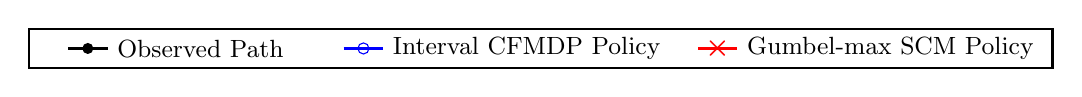
\begin{tikzpicture}[scale=1.0, every node/.style={scale=1.0}]
            \draw[thick, black] (-3, -0.25) rectangle (10, 0.25);
            %
            \draw[black, line width=1pt] (-2.5, 0.0) -- (-2,0.0);
            \fill[black] (-2.25,0.0) circle (2pt); %
            \node[right] at (-2,0.0) {\small Observed Path};
            
            %
            \draw[blue, line width=1pt] (1.0,0.0) -- (1.5,0.0);
            \node[draw=blue, circle, minimum size=4pt, inner sep=0pt] at (1.25,0.0) {}; %
            \node[right] at (1.5,0.0) {\small Interval CFMDP Policy};
            
            %
            \draw[red, line width=1pt] (5.5,0) -- (6,0);
            \node[red] at (5.75,0) {$\boldsymbol{\times}$}; %
            \node[right] at (6,0) {\small Gumbel-max SCM Policy};
        \end{tikzpicture}
    }\\
    %
    \subfigure[\footnotesize Lowest cumulative reward: Interval CFMDP ($312$), Gumbel-max SCM ($312$)]{%
        \resizebox{0.76\columnwidth}{!}{
             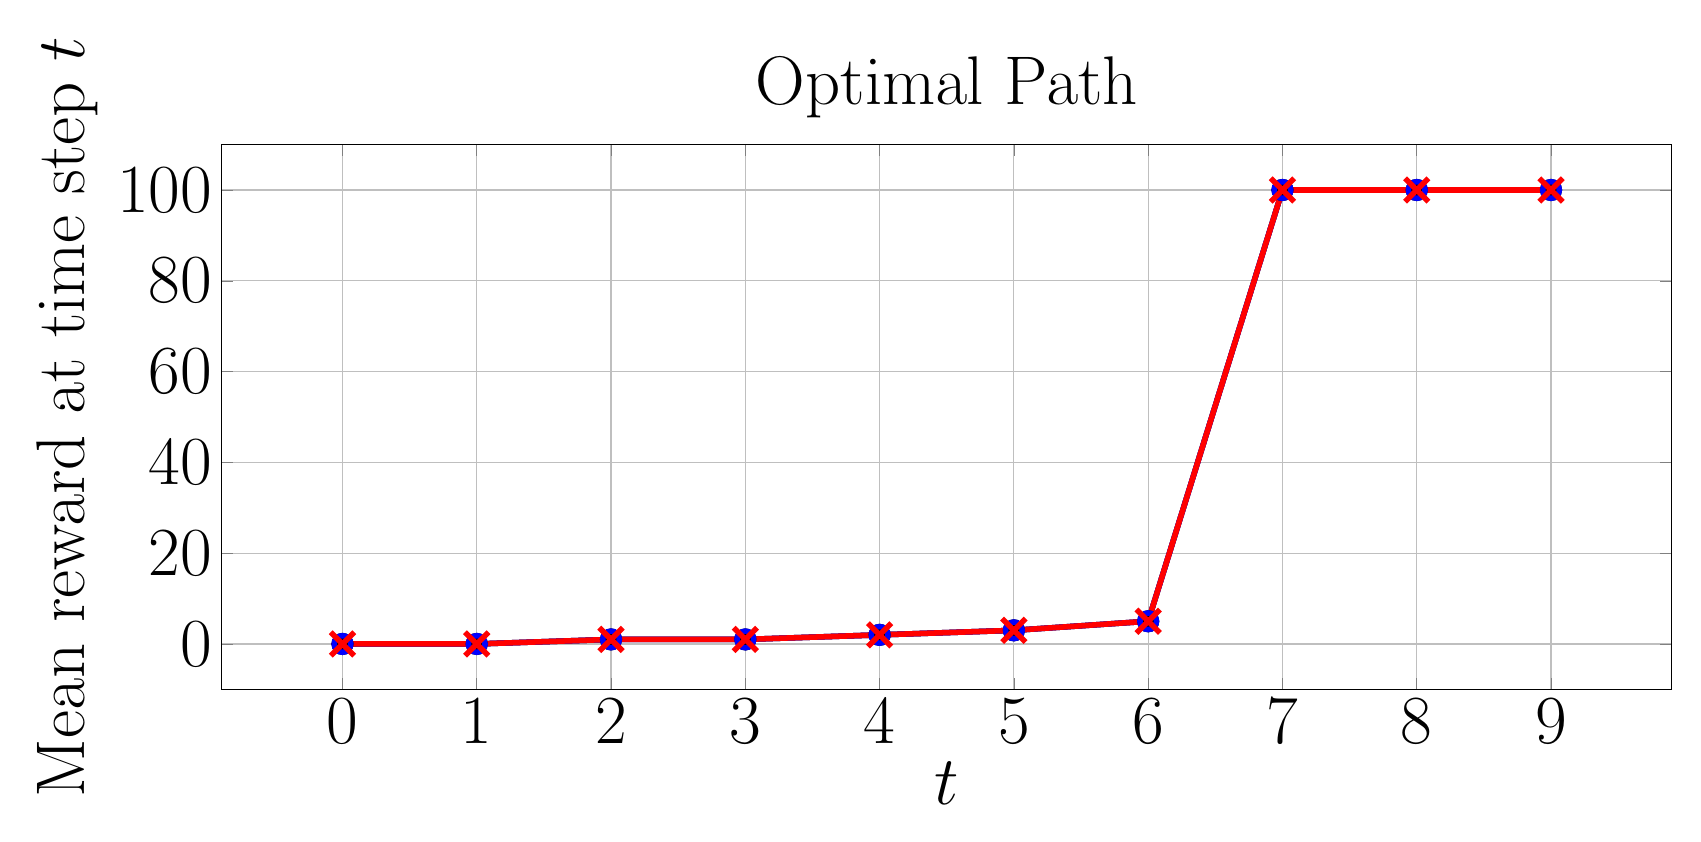
\begin{tikzpicture}
                \begin{axis}[
                    xlabel={$t$},
                    ylabel={Mean reward at time step $t$},
                    title={Optimal Path},
                    grid=both,
                    width=20cm, height=8.5cm,
                    every axis/.style={font=\Huge},
                    %
                ]
                \addplot[
                    color=black, %
                    mark=*, %
                    line width=2pt,
                    mark size=3pt,
                    error bars/.cd,
                    y dir=both, %
                    y explicit, %
                    error bar style={line width=1pt,solid},
                    error mark options={line width=1pt,mark size=4pt,rotate=90}
                ]
                coordinates {
                    (0, 0.0)  +- (0, 0.0)
                    (1, 0.0)  +- (0, 0.0) 
                    (2, 1.0)  +- (0, 0.0) 
                    (3, 1.0)  +- (0, 0.0)
                    (4, 2.0)  +- (0, 0.0)
                    (5, 3.0) +- (0, 0.0)
                    (6, 5.0) +- (0, 0.0)
                    (7, 100.0) +- (0, 0.0)
                    (8, 100.0) +- (0, 0.0)
                    (9, 100.0) +- (0, 0.0)
                };
                %
                \addplot[
                    color=blue, %
                    mark=o, %
                    line width=2pt,
                    mark size=3pt,
                    error bars/.cd,
                    y dir=both, %
                    y explicit, %
                    error bar style={line width=1pt,solid},
                    error mark options={line width=1pt,mark size=4pt,rotate=90}
                ]
                 coordinates {
                    (0, 0.0)  +- (0, 0.0)
                    (1, 0.0)  +- (0, 0.0) 
                    (2, 1.0)  +- (0, 0.0) 
                    (3, 1.0)  +- (0, 0.0)
                    (4, 2.0)  +- (0, 0.0)
                    (5, 3.0) +- (0, 0.0)
                    (6, 5.0) +- (0, 0.0)
                    (7, 100.0) +- (0, 0.0)
                    (8, 100.0) +- (0, 0.0)
                    (9, 100.0) +- (0, 0.0)
                };
                %
                \addplot[
                    color=red, %
                    mark=x, %
                    line width=2pt,
                    mark size=6pt,
                    error bars/.cd,
                    y dir=both, %
                    y explicit, %
                    error bar style={line width=1pt,solid},
                    error mark options={line width=1pt,mark size=4pt,rotate=90}
                ]
                coordinates {
                    (0, 0.0)  +- (0, 0.0)
                    (1, 0.0)  +- (0, 0.0) 
                    (2, 1.0)  +- (0, 0.0) 
                    (3, 1.0)  +- (0, 0.0)
                    (4, 2.0)  +- (0, 0.0)
                    (5, 3.0) +- (0, 0.0)
                    (6, 5.0) +- (0, 0.0)
                    (7, 100.0) +- (0, 0.0)
                    (8, 100.0) +- (0, 0.0)
                    (9, 100.0) +- (0, 0.0)
                };
                \end{axis}
            \end{tikzpicture}
         }
    }
    \hspace{1cm}
    \subfigure[\footnotesize Lowest cumulative reward: Interval CFMDP ($19$), Gumbel-max SCM ($-88$)]{%
         \resizebox{0.76\columnwidth}{!}{
            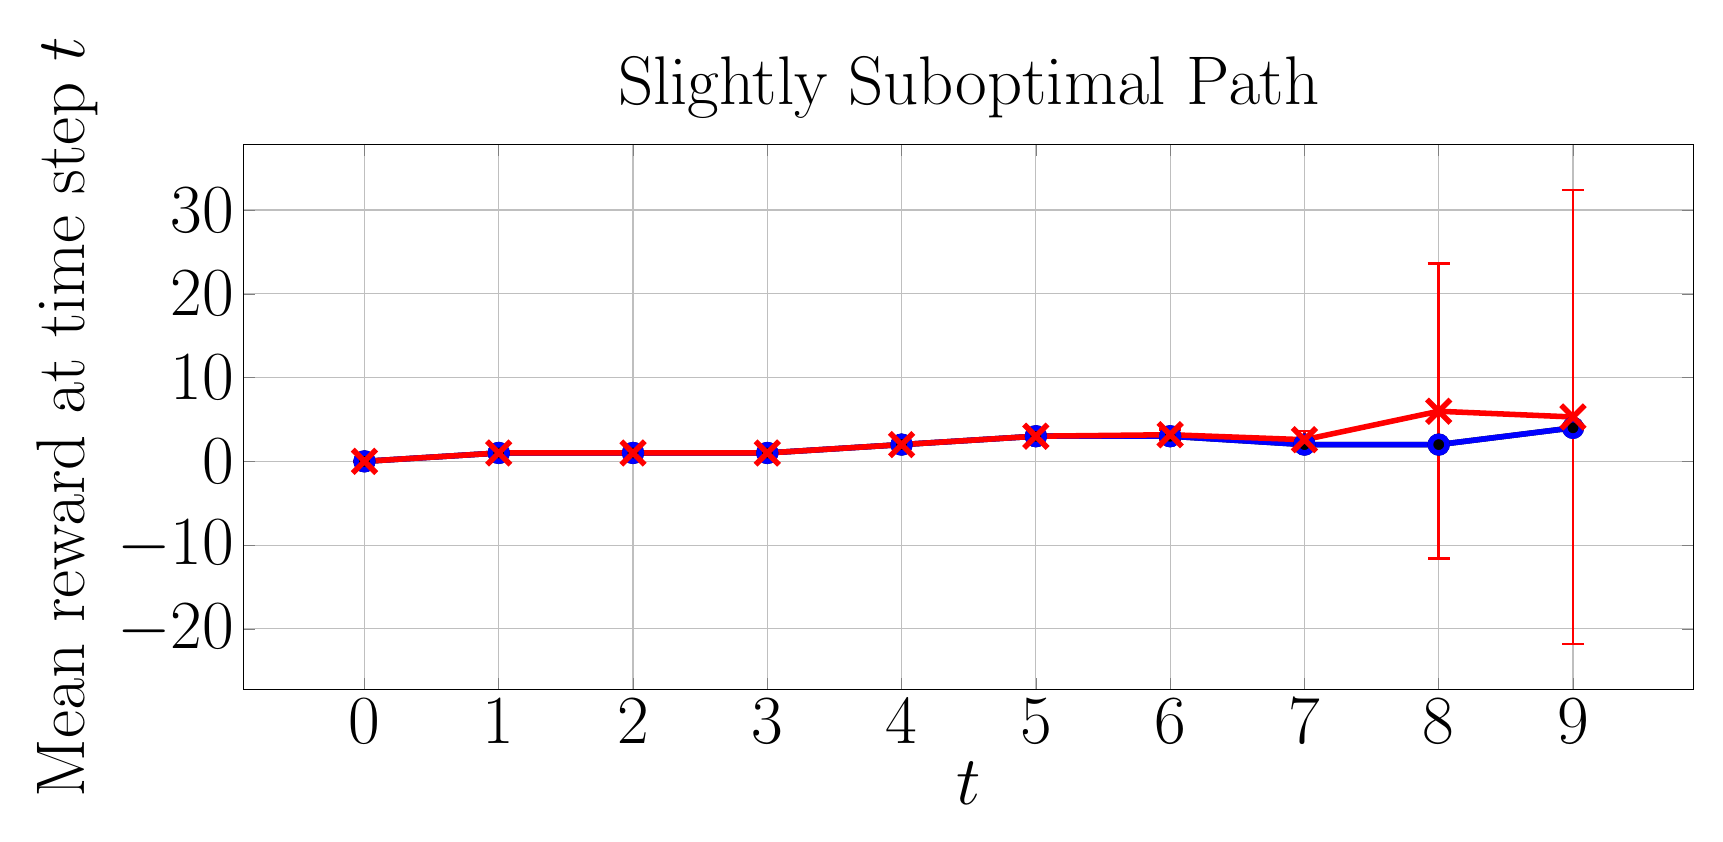
\begin{tikzpicture}
                \begin{axis}[
                    xlabel={$t$},
                    ylabel={Mean reward at time step $t$},
                    title={Slightly Suboptimal Path},
                    grid=both,
                    width=20cm, height=8.5cm,
                    every axis/.style={font=\Huge},
                    %
                ]
                \addplot[
                    color=black, %
                    mark=*, %
                    line width=2pt,
                    mark size=3pt,
                    error bars/.cd,
                    y dir=both, %
                    y explicit, %
                    error bar style={line width=1pt,solid},
                    error mark options={line width=1pt,mark size=4pt,rotate=90}
                ]
              coordinates {
                    (0, 0.0)  +- (0, 0.0)
                    (1, 1.0)  +- (0, 0.0) 
                    (2, 1.0)  +- (0, 0.0) 
                    (3, 1.0)  +- (0, 0.0)
                    (4, 2.0)  +- (0, 0.0)
                    (5, 3.0) +- (0, 0.0)
                    (6, 3.0) +- (0, 0.0)
                    (7, 2.0) +- (0, 0.0)
                    (8, 2.0) +- (0, 0.0)
                    (9, 4.0) +- (0, 0.0)
                };
                %
                \addplot[
                    color=blue, %
                    mark=o, %
                    line width=2pt,
                    mark size=3pt,
                    error bars/.cd,
                    y dir=both, %
                    y explicit, %
                    error bar style={line width=1pt,solid},
                    error mark options={line width=1pt,mark size=4pt,rotate=90}
                ]
              coordinates {
                    (0, 0.0)  +- (0, 0.0)
                    (1, 1.0)  +- (0, 0.0) 
                    (2, 1.0)  +- (0, 0.0) 
                    (3, 1.0)  +- (0, 0.0)
                    (4, 2.0)  +- (0, 0.0)
                    (5, 3.0) +- (0, 0.0)
                    (6, 3.0) +- (0, 0.0)
                    (7, 2.0) +- (0, 0.0)
                    (8, 2.0) +- (0, 0.0)
                    (9, 4.0) +- (0, 0.0)
                };
                %
                \addplot[
                    color=red, %
                    mark=x, %
                    line width=2pt,
                    mark size=6pt,
                    error bars/.cd,
                    y dir=both, %
                    y explicit, %
                    error bar style={line width=1pt,solid},
                    error mark options={line width=1pt,mark size=4pt,rotate=90}
                ]
                coordinates {
                    (0, 0.0)  +- (0, 0.0)
                    (1, 1.0)  +- (0, 0.0) 
                    (2, 1.0)  +- (0, 0.0) 
                    (3, 1.0)  +- (0, 0.0)
                    (4, 2.0)  += (0, 0.0)
                    (5, 3.0)  += (0, 0.0)
                    (6, 3.17847) += (0, 0.62606746) -= (0, 0.62606746)
                    (7, 2.5832885) += (0, 1.04598233) -= (0, 1.04598233)
                    (8, 5.978909) += (0, 17.60137623) -= (0, 17.60137623)
                    (9, 5.297059) += (0, 27.09227512) -= (0, 27.09227512)
                };
                \end{axis}
            \end{tikzpicture}
         }
    }\\[-1.5pt]
    \subfigure[\footnotesize Lowest cumulative reward: Interval CFMDP ($14$), Gumbel-max SCM ($-598$)]{%
         \resizebox{0.76\columnwidth}{!}{
             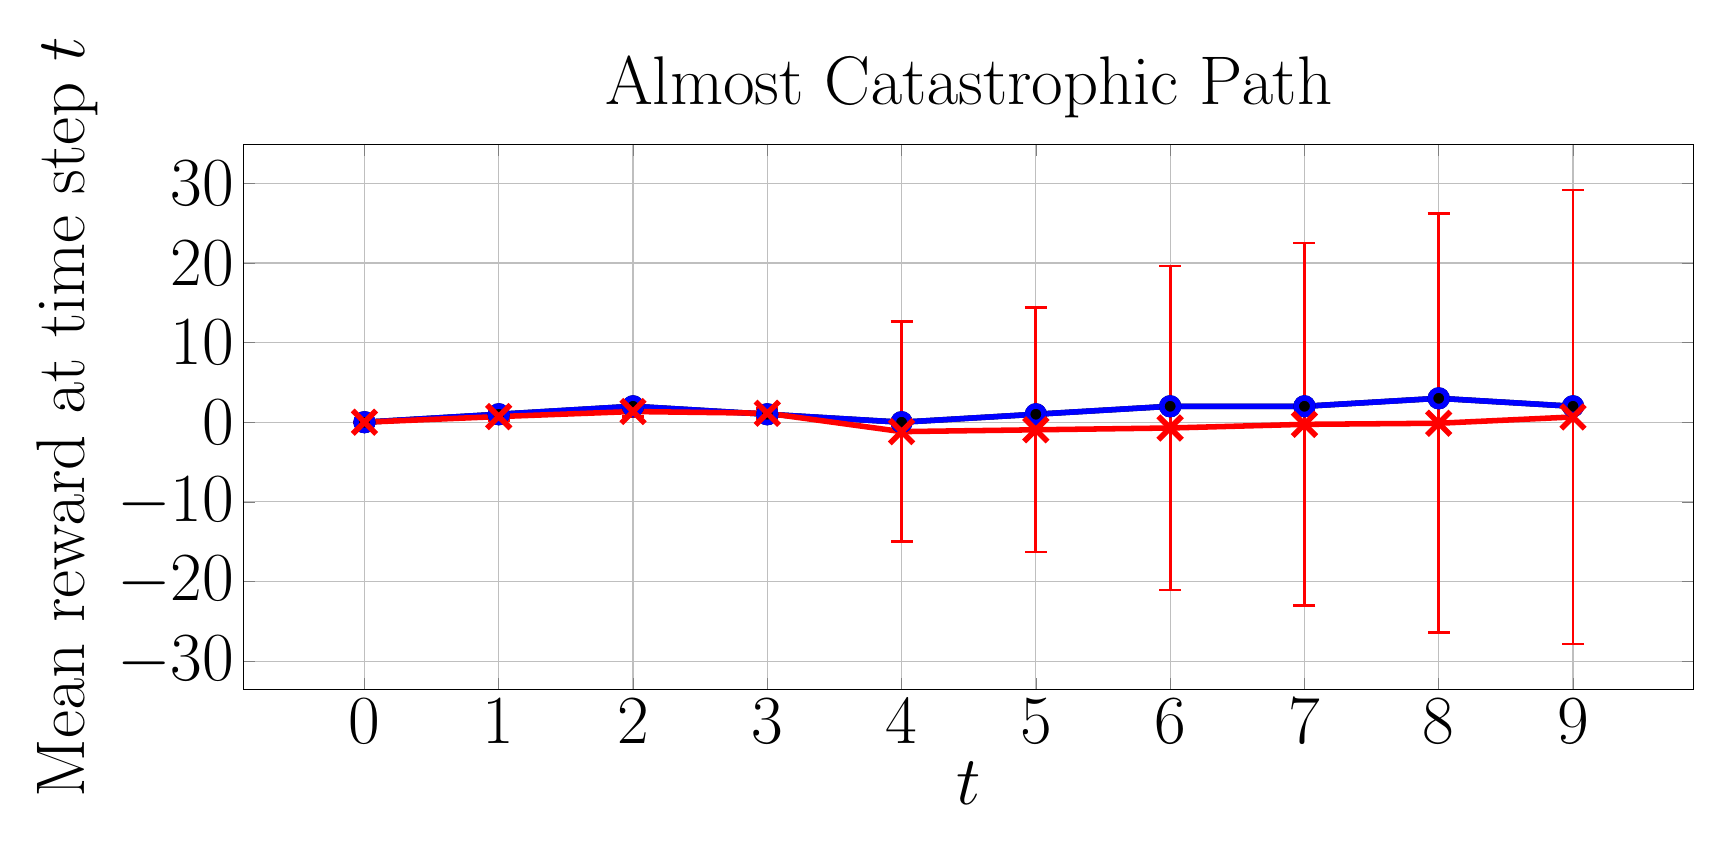
\begin{tikzpicture}
                \begin{axis}[
                    xlabel={$t$},
                    ylabel={Mean reward at time step $t$},
                    title={Almost Catastrophic Path},
                    grid=both,
                    width=20cm, height=8.5cm,
                    every axis/.style={font=\Huge},
                    %
                ]
                \addplot[
                    color=black, %
                    mark=*, %
                    line width=2pt,
                    mark size=3pt,
                    error bars/.cd,
                    y dir=both, %
                    y explicit, %
                    error bar style={line width=1pt,solid},
                    error mark options={line width=1pt,mark size=4pt,rotate=90}
                ]
                coordinates {
                    (0, 0.0)  +- (0, 0.0)
                    (1, 1.0)  +- (0, 0.0) 
                    (2, 2.0)  +- (0, 0.0) 
                    (3, 1.0)  +- (0, 0.0)
                    (4, 0.0)  +- (0, 0.0)
                    (5, 1.0) +- (0, 0.0)
                    (6, 2.0) +- (0, 0.0)
                    (7, 2.0) +- (0, 0.0)
                    (8, 3.0) +- (0, 0.0)
                    (9, 2.0) +- (0, 0.0)
                };
                %
                \addplot[
                    color=blue, %
                    mark=o, %
                    line width=2pt,
                    mark size=3pt,
                    error bars/.cd,
                    y dir=both, %
                    y explicit, %
                    error bar style={line width=1pt,solid},
                    error mark options={line width=1pt,mark size=4pt,rotate=90}
                ]
                coordinates {
                    (0, 0.0)  +- (0, 0.0)
                    (1, 1.0)  +- (0, 0.0) 
                    (2, 2.0)  +- (0, 0.0) 
                    (3, 1.0)  +- (0, 0.0)
                    (4, 0.0)  +- (0, 0.0)
                    (5, 1.0) +- (0, 0.0)
                    (6, 2.0) +- (0, 0.0)
                    (7, 2.0) +- (0, 0.0)
                    (8, 3.0) +- (0, 0.0)
                    (9, 2.0) +- (0, 0.0)
                };
                %
                \addplot[
                    color=red, %
                    mark=x, %
                    line width=2pt,
                    mark size=6pt,
                    error bars/.cd,
                    y dir=both, %
                    y explicit, %
                    error bar style={line width=1pt,solid},
                    error mark options={line width=1pt,mark size=4pt,rotate=90}
                ]
                coordinates {
                    (0, 0.0)  +- (0, 0.0)
                    (1, 0.7065655)  +- (0, 0.4553358) 
                    (2, 1.341673)  +- (0, 0.67091621) 
                    (3, 1.122926)  +- (0, 0.61281824)
                    (4, -1.1821935)  +- (0, 13.82444042)
                    (5, -0.952399)  +- (0, 15.35195457)
                    (6, -0.72672) +- (0, 20.33508414)
                    (7, -0.268983) +- (0, 22.77861454)
                    (8, -0.1310835) +- (0, 26.31013314)
                    (9, 0.65806) +- (0, 28.50670214)
                };
                %
            %
            %
            %
            %
            %
            %
            %
            %
            %
            %
            %
            %
            %
            %
            %
            %
            %
            %
                \end{axis}
            \end{tikzpicture}
         }
    }
    \hspace{1cm}
    \subfigure[\footnotesize Lowest cumulative reward: Interval CFMDP ($-698$), Gumbel-max SCM ($-698$)]{%
         \resizebox{0.76\columnwidth}{!}{
            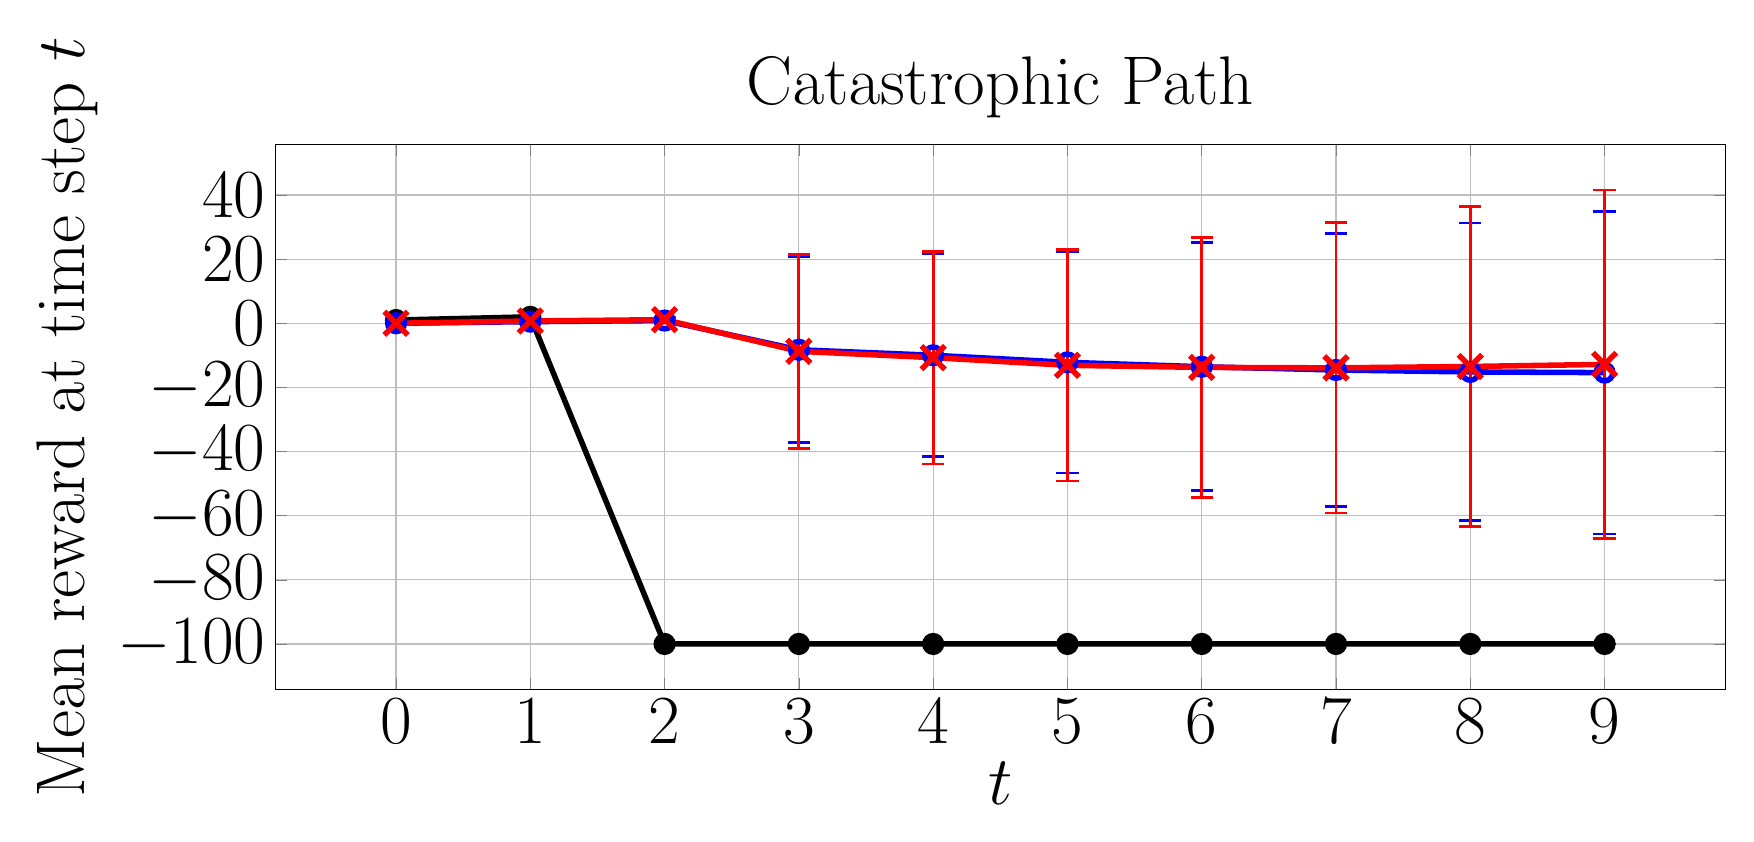
\begin{tikzpicture}
                \begin{axis}[
                    xlabel={$t$},
                    ylabel={Mean reward at time step $t$},
                    title={Catastrophic Path},
                    grid=both,
                    width=20cm, height=8.5cm,
                    every axis/.style={font=\Huge},
                    %
                ]
                \addplot[
                    color=black, %
                    mark=*, %
                    line width=2pt,
                    mark size=3pt,
                    error bars/.cd,
                    y dir=both, %
                    y explicit, %
                    error bar style={line width=1pt,solid},
                    error mark options={line width=1pt,mark size=4pt,rotate=90}
                ]
                coordinates {
                    (0, 1.0)  +- (0, 0.0)
                    (1, 2.0)  +- (0, 0.0) 
                    (2, -100.0)  +- (0, 0.0) 
                    (3, -100.0)  +- (0, 0.0)
                    (4, -100.0)  +- (0, 0.0)
                    (5, -100.0) +- (0, 0.0)
                    (6, -100.0) +- (0, 0.0)
                    (7, -100.0) +- (0, 0.0)
                    (8, -100.0) +- (0, 0.0)
                    (9, -100.0) +- (0, 0.0)
                };
                %
                \addplot[
                    color=blue, %
                    mark=o, %
                    line width=2pt,
                    mark size=3pt,
                    error bars/.cd,
                    y dir=both, %
                    y explicit, %
                    error bar style={line width=1pt,solid},
                    error mark options={line width=1pt,mark size=4pt,rotate=90}
                ]
                coordinates {
                    (0, 0.0)  +- (0, 0.0)
                    (1, 0.504814)  +- (0, 0.49997682) 
                    (2, 0.8439835)  +- (0, 0.76831917) 
                    (3, -8.2709165)  +- (0, 28.93656754)
                    (4, -9.981082)  +- (0, 31.66825363)
                    (5, -12.1776325) +- (0, 34.53463233)
                    (6, -13.556076) +- (0, 38.62845372)
                    (7, -14.574418) +- (0, 42.49603359)
                    (8, -15.1757075) +- (0, 46.41913968)
                    (9, -15.3900395) +- (0, 50.33563368)
                };
                %
                \addplot[
                    color=red, %
                    mark=x, %
                    line width=2pt,
                    mark size=6pt,
                    error bars/.cd,
                    y dir=both, %
                    y explicit, %
                    error bar style={line width=1pt,solid},
                    error mark options={line width=1pt,mark size=4pt,rotate=90}
                ]
                coordinates {
                    (0, 0.0)  +- (0, 0.0)
                    (1, 0.701873)  +- (0, 0.45743556) 
                    (2, 1.1227805)  +- (0, 0.73433129) 
                    (3, -8.7503255)  +- (0, 30.30257976)
                    (4, -10.722092)  +- (0, 33.17618589)
                    (5, -13.10721)  +- (0, 36.0648089)
                    (6, -13.7631645) +- (0, 40.56553451)
                    (7, -13.909043) +- (0, 45.23829402)
                    (8, -13.472517) +- (0, 49.96270296)
                    (9, -12.8278835) +- (0, 54.38618735)
                };
                %
            %
            %
            %
            %
            %
            %
            %
            %
            %
            %
            %
            %
            %
            %
            %
            %
            %
            %
                \end{axis}
            \end{tikzpicture}
         }
    }
    \caption{Average instant reward of CF paths induced by policies on GridWorld $p=0.4$.}
    \label{fig: reward p=0.4}
\end{figure*}

\subsection{Experimental Setup}
To compare policy performance, we measure the average rewards of counterfactual paths induced by our policy and the Gumbel-max policy by uniformly sampling $200$ counterfactual MDPs from the ICFMDP and generating $10,000$ counterfactual paths over each sampled CFMDP. \jl{Since the interval CFMDP depends on the observed path, we select $4$  paths of varying optimality to evaluate how the observed path impacts the performance of both policies: an optimal path, a slightly suboptimal path that could reach the optimal reward with a few changes, a catastrophic path that enters a catastrophic, terminal state with low reward, and an almost catastrophic path that was close to entering a catastrophic state.} When measuring the average probability bound widths and execution time needed to generate the ICFMDPs, we averaged over $20$ randomly generated observed paths
\footnote{Further training details are provided in Appendix \ref{app: training details}, and the code is provided at \href{https://github.com/ddv-lab/robust-cf-inference-in-MDPs}{https://github.com/ddv-lab/robust-cf-inference-in-MDPs}
%
%
.}.

\subsection{GridWorld}
\jl{The GridWorld MDP is a $4 \times 4$ grid where an agent must navigate from the top-left corner to the goal state in the bottom-right corner, avoiding a dangerous terminal state in the centre. At each time step, the agent can move up, down, left, or right, but there is a small probability (controlled by hyper-parameter $p$) of moving in an unintended direction. As the agent nears the goal, the reward for each state increases, culminating in a reward of $+100$ for reaching the goal. Entering the dangerous state results in a penalty of $-100$. We use two versions of GridWorld: a less stochastic version with $p=0.9$ (i.e., $90$\% chance of moving in the chosen direction) and a more stochastic version with $p=0.4$.}

\paragraph{GridWorld ($p=0.9$)}
When $p=0.9$, the counterfactual probability bounds are typically narrow (see Table \ref{tab:nonzero_probs} for average measurements). Consequently, as shown in Figure \ref{fig: reward p=0.9}, both policies are nearly identical and perform similarly well across the optimal, slightly suboptimal, and catastrophic paths.
%
However, for the almost catastrophic path, the interval CFMDP path is more conservative and follows the observed path more closely (as this is where the probability bounds are narrowest), which typically requires one additional step to reach the goal state than the Gumbel-max SCM policy.
%

\paragraph{GridWorld ($p=0.4$)}
\jl{When $p=0.4$, the GridWorld environment becomes more uncertain, increasing the risk of entering the dangerous state even if correct actions are chosen. Thus, as shown in Figure \ref{fig: reward p=0.4}, the interval CFMDP policy adopts a more conservative approach, avoiding deviation from the observed policy if it cannot guarantee higher counterfactual rewards (see the slightly suboptimal and almost catastrophic paths), whereas the Gumbel-max SCM is inconsistent: it can yield higher rewards, but also much lower rewards, reflected in the wide error bars.} For the catastrophic path, both policies must deviate from the observed path to achieve a higher reward and, in this case, perform similarly.
%
%
%
%
\subsection{Sepsis}
The Sepsis MDP \citep{oberst2019counterfactual} simulates trajectories of Sepsis patients. Each state consists of four vital signs (heart rate, blood pressure, oxygen concentration, and glucose levels), categorised as low, normal, or high.
and three treatments that can be toggled on/off at each time step (8 actions in total). Unlike \citet{oberst2019counterfactual}, we scale rewards based on the number of out-of-range vital signs, between $-1000$ (patient dies) and $1000$ (patient discharged). \jl{Like the GridWorld $p=0.4$ experiment, the Sepsis MDP is highly uncertain, as many states are equally likely to lead to optimal and poor outcomes. Thus, as shown in Figure \ref{fig: reward sepsis}, both policies follow the observed optimal and almost catastrophic paths to guarantee rewards are no worse than the observation.} However, improving the catastrophic path requires deviating from the observation. Here, the Gumbel-max SCM policy, on average, performs better than the interval CFMDP policy. But, since both policies have lower bounds clipped at $-1000$, neither policy reliably improves over the observation. In contrast, for the slightly suboptimal path, the interval CFMDP policy performs significantly better, shown by its higher lower bounds. 
Moreover, in these two cases, the worst-case counterfactual path generated by the interval CFMDP policy is better than that of the Gumbel-max SCM policy,
indicating its greater robustness.
%
\begin{figure*}
    \centering
     \resizebox{0.6\textwidth}{!}{
        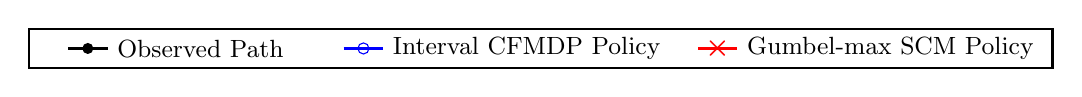
\begin{tikzpicture}[scale=1.0, every node/.style={scale=1.0}]
            \draw[thick, black] (-3, -0.25) rectangle (10, 0.25);
            %
            \draw[black, line width=1pt] (-2.5, 0.0) -- (-2,0.0);
            \fill[black] (-2.25,0.0) circle (2pt); %
            \node[right] at (-2,0.0) {\small Observed Path};
            
            %
            \draw[blue, line width=1pt] (1.0,0.0) -- (1.5,0.0);
            \node[draw=blue, circle, minimum size=4pt, inner sep=0pt] at (1.25,0.0) {}; %
            \node[right] at (1.5,0.0) {\small Interval CFMDP Policy};
            
            %
            \draw[red, line width=1pt] (5.5,0) -- (6,0);
            \node[red] at (5.75,0) {$\boldsymbol{\times}$}; %
            \node[right] at (6,0) {\small Gumbel-max SCM Policy};
        \end{tikzpicture}
    }\\
    \subfigure[\footnotesize Lowest cumulative reward: Interval CFMDP ($8000$), Gumbel-max SCM ($8000$)]{%
         \resizebox{0.76\columnwidth}{!}{
             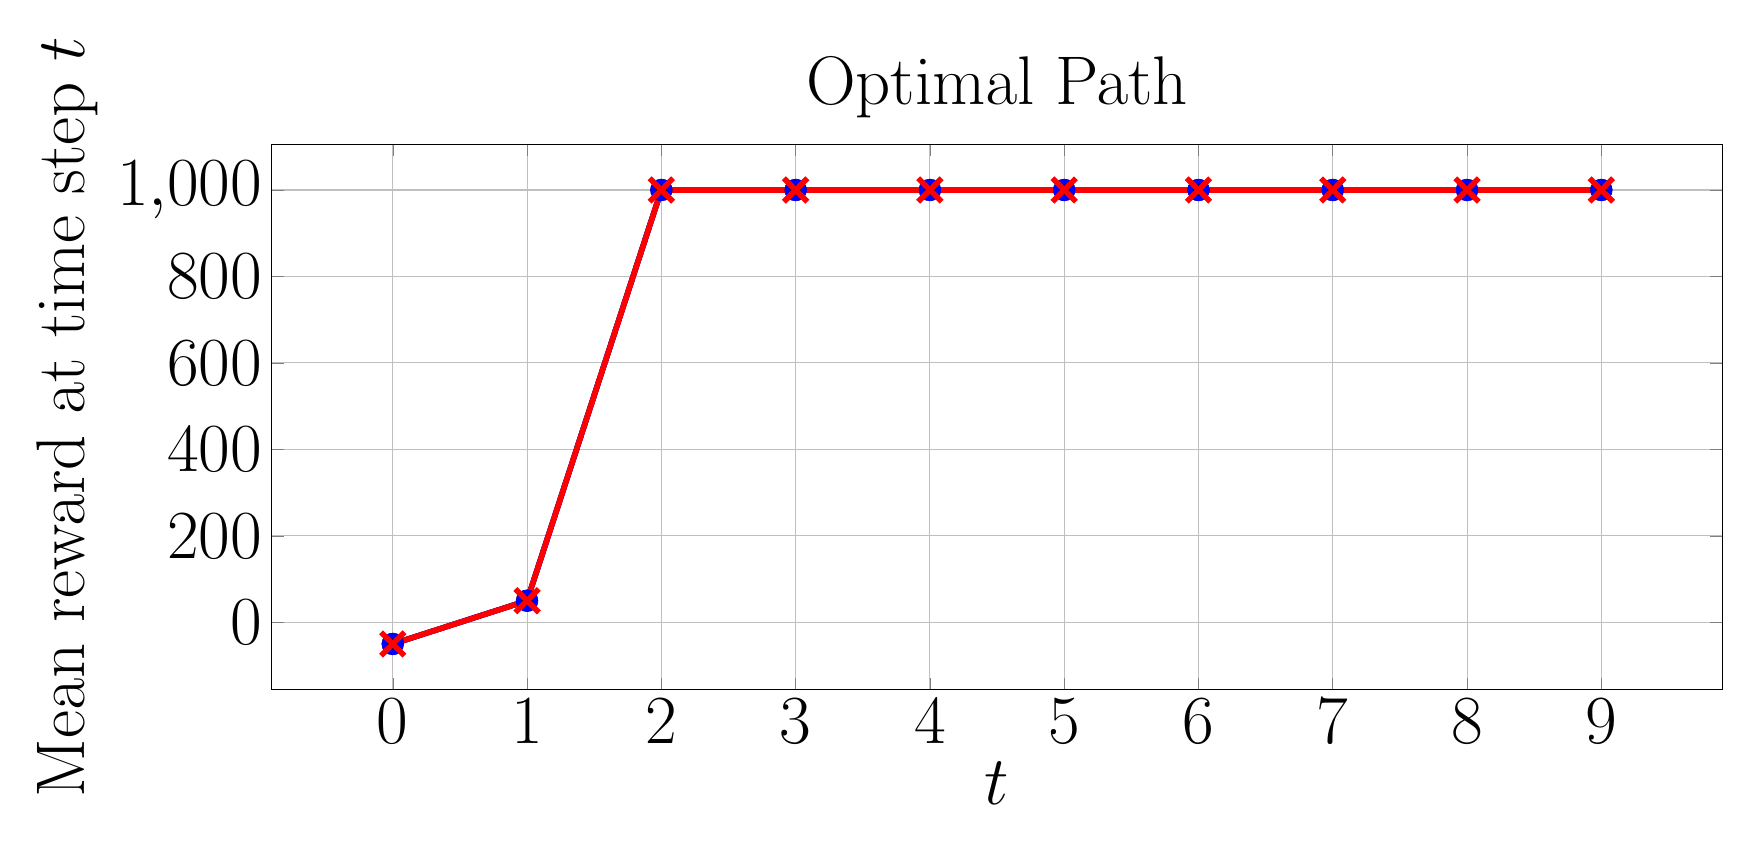
\begin{tikzpicture}
                \begin{axis}[
                    xlabel={$t$},
                    ylabel={Mean reward at time step $t$},
                    title={Optimal Path},
                    grid=both,
                    width=20cm, height=8.5cm,
                    every axis/.style={font=\Huge},
                    %
                ]
                \addplot[
                    color=black, %
                    mark=*, %
                    line width=2pt,
                    mark size=3pt,
                ]
                coordinates {
                    (0, -50.0)
                    (1, 50.0)
                    (2, 1000.0)
                    (3, 1000.0)
                    (4, 1000.0)
                    (5, 1000.0)
                    (6, 1000.0)
                    (7, 1000.0)
                    (8, 1000.0)
                    (9, 1000.0)
                };
                %
                \addplot[
                    color=blue, %
                    mark=o, %
                    line width=2pt,
                    mark size=3pt,
                    error bars/.cd,
                    y dir=both, %
                    y explicit, %
                    error bar style={line width=1pt,solid},
                    error mark options={line width=1pt,mark size=4pt,rotate=90}
                ]
                coordinates {
                    (0, -50.0)  +- (0, 0.0)
                    (1, 50.0)  +- (0, 0.0) 
                    (2, 1000.0)  +- (0, 0.0) 
                    (3, 1000.0)  +- (0, 0.0)
                    (4, 1000.0)  +- (0, 0.0)
                    (5, 1000.0) +- (0, 0.0)
                    (6, 1000.0) +- (0, 0.0)
                    (7, 1000.0) +- (0, 0.0)
                    (8, 1000.0) +- (0, 0.0)
                    (9, 1000.0) +- (0, 0.0)
                };
                %
                \addplot[
                    color=red, %
                    mark=x, %
                    line width=2pt,
                    mark size=6pt,
                    error bars/.cd,
                    y dir=both, %
                    y explicit, %
                    error bar style={line width=1pt,solid},
                    error mark options={line width=1pt,mark size=4pt,rotate=90}
                ]
                coordinates {
                    (0, -50.0)  +- (0, 0.0)
                    (1, 50.0)  +- (0, 0.0) 
                    (2, 1000.0)  +- (0, 0.0) 
                    (3, 1000.0)  +- (0, 0.0)
                    (4, 1000.0)  +- (0, 0.0)
                    (5, 1000.0) +- (0, 0.0)
                    (6, 1000.0) +- (0, 0.0)
                    (7, 1000.0) +- (0, 0.0)
                    (8, 1000.0) +- (0, 0.0)
                    (9, 1000.0) +- (0, 0.0)
                };
                %
                \end{axis}
            \end{tikzpicture}
         }
    }
    \hspace{1cm}
    \subfigure[\footnotesize Lowest cumulative reward: Interval CFMDP ($-5980$), Gumbel-max SCM ($-8000$)]{%
         \resizebox{0.76\columnwidth}{!}{
            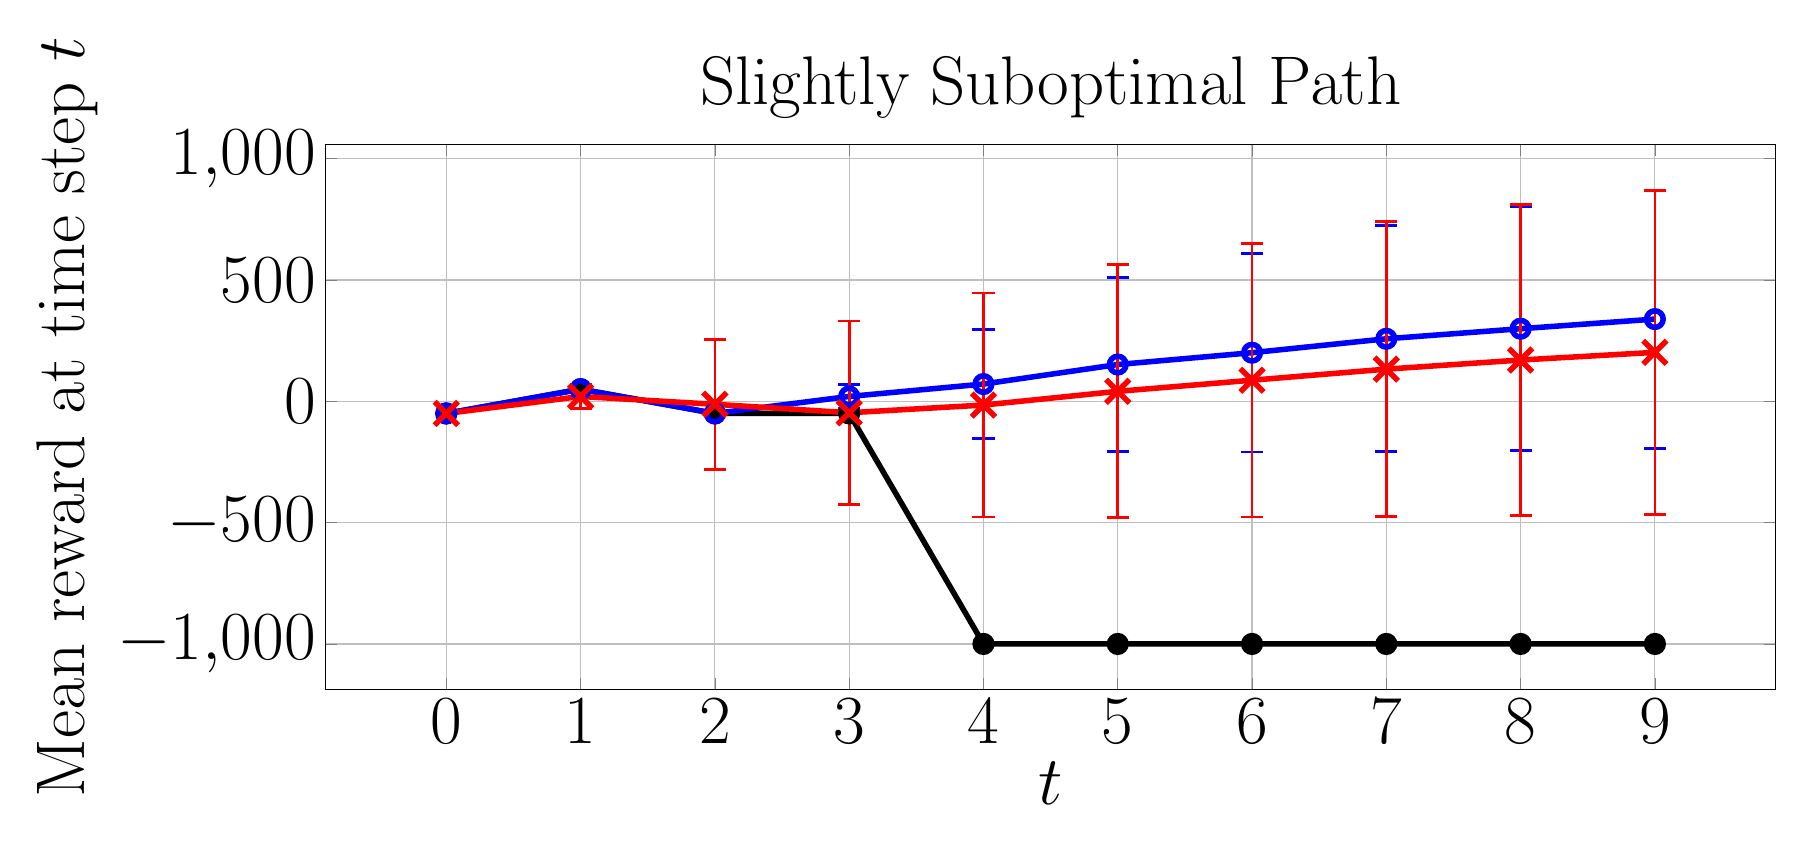
\begin{tikzpicture}
                \begin{axis}[
                    xlabel={$t$},
                    ylabel={Mean reward at time step $t$},
                    title={Slightly Suboptimal Path},
                    grid=both,
                    width=20cm, height=8.5cm,
                    every axis/.style={font=\Huge},
                    %
                ]
               \addplot[
                    color=black, %
                    mark=*, %
                    line width=2pt,
                    mark size=3pt,
                ]
                coordinates {
                    (0, -50.0)
                    (1, 50.0)
                    (2, -50.0)
                    (3, -50.0)
                    (4, -1000.0)
                    (5, -1000.0)
                    (6, -1000.0)
                    (7, -1000.0)
                    (8, -1000.0)
                    (9, -1000.0)
                };
                %
                \addplot[
                    color=blue, %
                    mark=o, %
                    line width=2pt,
                    mark size=3pt,
                    error bars/.cd,
                    y dir=both, %
                    y explicit, %
                    error bar style={line width=1pt,solid},
                    error mark options={line width=1pt,mark size=4pt,rotate=90}
                ]
                coordinates {
                    (0, -50.0)  +- (0, 0.0)
                    (1, 50.0)  +- (0, 0.0) 
                    (2, -50.0)  +- (0, 0.0) 
                    (3, 20.0631)  +- (0, 49.97539413)
                    (4, 71.206585)  +- (0, 226.02033693)
                    (5, 151.60797) +- (0, 359.23292559)
                    (6, 200.40593) +- (0, 408.86185176)
                    (7, 257.77948) +- (0, 466.10372804)
                    (8, 299.237465) +- (0, 501.82579506)
                    (9, 338.9129) +- (0, 532.06124996)
                };
                %
                \addplot[
                    color=red, %
                    mark=x, %
                    line width=2pt,
                    mark size=6pt,
                    error bars/.cd,
                    y dir=both, %
                    y explicit, %
                    error bar style={line width=1pt,solid},
                    error mark options={line width=1pt,mark size=4pt,rotate=90}
                ]
                coordinates {
                    (0, -50.0)  +- (0, 0.0)
                    (1, 20.00736)  +- (0, 49.99786741) 
                    (2, -12.282865)  +- (0, 267.598755) 
                    (3, -47.125995)  +- (0, 378.41755832)
                    (4, -15.381965)  +- (0, 461.77616558)
                    (5, 41.15459) +- (0, 521.53189262)
                    (6, 87.01595) +- (0, 564.22243126 )
                    (7, 132.62376) +- (0, 607.31338037)
                    (8, 170.168145) +- (0, 641.48013693)
                    (9, 201.813135) +- (0, 667.29441777)
                };
                %
                %
                %
                %
                %
                %
                %
                %
                %
                %
                %
                %
                %
                %
                %
                %
                %
                %
                %
                \end{axis}
            \end{tikzpicture}
         }
    }\\[-1.5pt]
    \subfigure[\footnotesize Lowest cumulative reward: Interval CFMDP ($100$), Gumbel-max SCM ($100$)]{%
         \resizebox{0.76\columnwidth}{!}{
             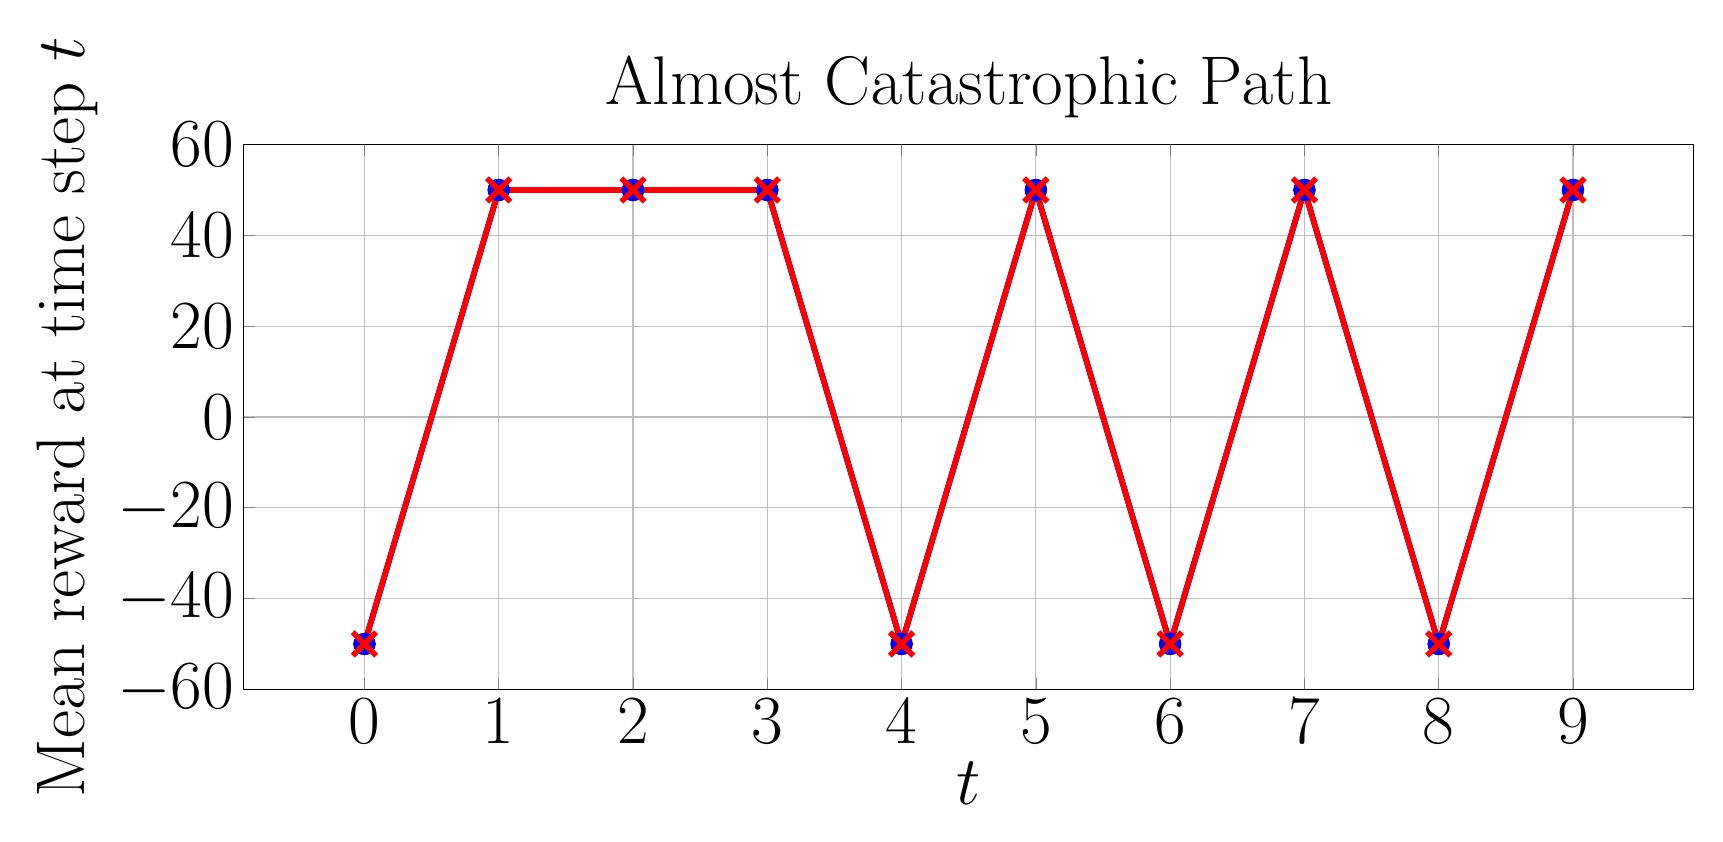
\begin{tikzpicture}
                \begin{axis}[
                    xlabel={$t$},
                    ylabel={Mean reward at time step $t$},
                    title={Almost Catastrophic Path},
                    grid=both,
                    every axis/.style={font=\Huge},
                    width=20cm, height=8.5cm,
                    %
                ]
               \addplot[
                    color=black, %
                    mark=*, %
                    line width=2pt,
                    mark size=3pt,
                ]
                coordinates {
                    (0, -50.0)
                    (1, 50.0)
                    (2, 50.0)
                    (3, 50.0)
                    (4, -50.0)
                    (5, 50.0)
                    (6, -50.0)
                    (7, 50.0)
                    (8, -50.0)
                    (9, 50.0)
                };
                %
                %
                \addplot[
                    color=blue, %
                    mark=o, %
                    line width=2pt,
                    mark size=3pt,
                    error bars/.cd,
                    y dir=both, %
                    y explicit, %
                    error bar style={line width=1pt,solid},
                    error mark options={line width=1pt,mark size=4pt,rotate=90}
                ]
                coordinates {
                    (0, -50.0)  +- (0, 0.0)
                    (1, 50.0)  +- (0, 0.0) 
                    (2, 50.0)  +- (0, 0.0) 
                    (3, 50.0)  +- (0, 0.0)
                    (4, -50.0)  +- (0, 0.0)
                    (5, 50.0) +- (0, 0.0)
                    (6, -50.0) +- (0, 0.0)
                    (7, 50.0) +- (0, 0.0)
                    (8, -50.0) +- (0, 0.0)
                    (9, 50.0) +- (0, 0.0)
                };
                %
                \addplot[
                    color=red, %
                    mark=x, %
                    line width=2pt,
                    mark size=6pt,
                    error bars/.cd,
                    y dir=both, %
                    y explicit, %
                    error bar style={line width=1pt,solid},
                    error mark options={line width=1pt,mark size=4pt,rotate=90}
                ]
                coordinates {
                    (0, -50.0)  +- (0, 0.0)
                    (1, 50.0)  +- (0, 0.0) 
                    (2, 50.0)  +- (0, 0.0) 
                    (3, 50.0)  +- (0, 0.0)
                    (4, -50.0)  +- (0, 0.0)
                    (5, 50.0) +- (0, 0.0)
                    (6, -50.0) +- (0, 0.0)
                    (7, 50.0) +- (0, 0.0)
                    (8, -50.0) +- (0, 0.0)
                    (9, 50.0) +- (0, 0.0)
                };
                %
                %
                %
                %
                %
                %
                %
                %
                %
                %
                %
                %
                %
                %
                %
                %
                %
                %
                %
                \end{axis}
            \end{tikzpicture}
         }
    }
    \hspace{1cm}
    \subfigure[\footnotesize Lowest cumulative reward: Interval CFMDP ($-7150$), Gumbel-max SCM ($-9050$)]{%
         \resizebox{0.76\columnwidth}{!}{
            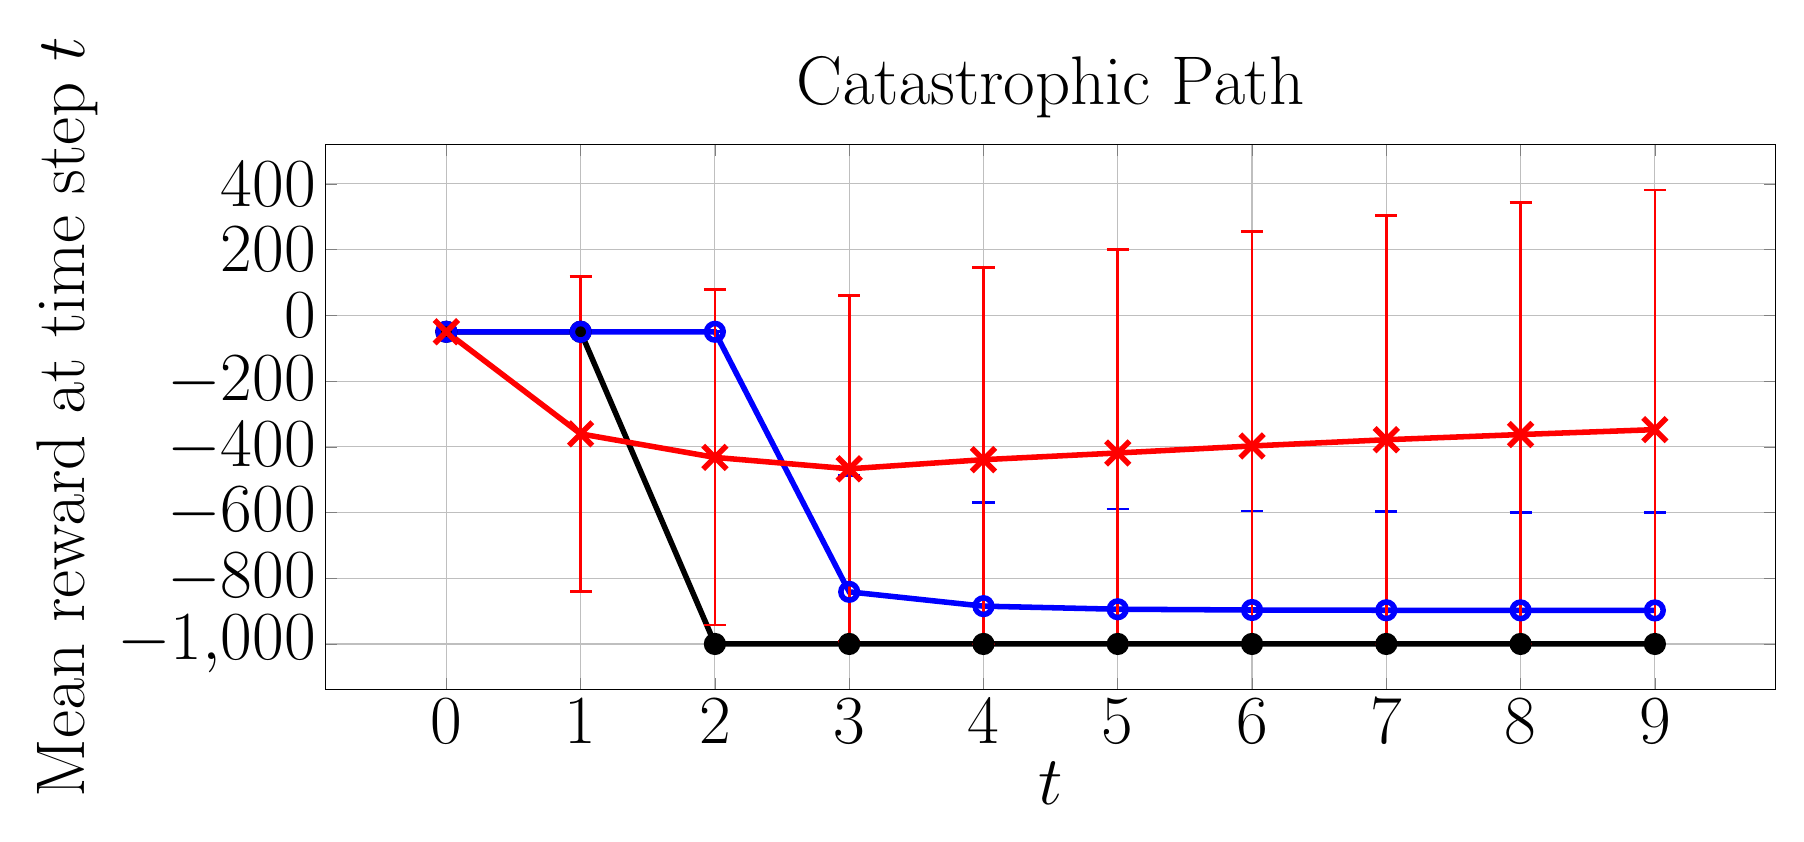
\begin{tikzpicture}
                \begin{axis}[
                    xlabel={$t$},
                    ylabel={Mean reward at time step $t$},
                    title={Catastrophic Path},
                    grid=both,
                    width=20cm, height=8.5cm,
                    every axis/.style={font=\Huge},
                    %
                ]
               \addplot[
                    color=black, %
                    mark=*, %
                    line width=2pt,
                    mark size=3pt,
                ]
                coordinates {
                    (0, -50.0)
                    (1, -50.0)
                    (2, -1000.0)
                    (3, -1000.0)
                    (4, -1000.0)
                    (5, -1000.0)
                    (6, -1000.0)
                    (7, -1000.0)
                    (8, -1000.0)
                    (9, -1000.0)
                };
                %
                %
                \addplot[
                    color=blue, %
                    mark=o, %
                    line width=2pt,
                    mark size=3pt,
                    error bars/.cd,
                    y dir=both, %
                    y explicit, %
                    error bar style={line width=1pt,solid},
                    error mark options={line width=1pt,mark size=4pt,rotate=90}
                ]
                coordinates {
                    (0, -50.0)  +- (0, 0.0)
                    (1, -50.0)  +- (0, 0.0) 
                    (2, -50.0)  +- (0, 0.0) 
                    (3, -841.440725)  += (0, 354.24605512) -= (0, 158.559275)
                    (4, -884.98225)  += (0, 315.37519669) -= (0, 115.01775)
                    (5, -894.330425) += (0, 304.88572805) -= (0, 105.669575)
                    (6, -896.696175) += (0, 301.19954514) -= (0, 103.303825)
                    (7, -897.4635) += (0, 299.61791279) -= (0, 102.5365)
                    (8, -897.77595) += (0, 298.80392585) -= (0, 102.22405)
                    (9, -897.942975) += (0, 298.32920557) -= (0, 102.057025)
                };
                %
                \addplot[
                    color=red, %
                    mark=x, %
                    line width=2pt,
                    mark size=6pt,
                    error bars/.cd,
                    y dir=both, %
                    y explicit, %
                    error bar style={line width=1pt,solid},
                    error mark options={line width=1pt,mark size=4pt,rotate=90}
                ]
            coordinates {
                    (0, -50.0)  +- (0, 0.0)
                    (1, -360.675265)  +- (0, 479.39812699) 
                    (2, -432.27629)  +- (0, 510.38620897) 
                    (3, -467.029545)  += (0, 526.36009628) -= (0, 526.36009628)
                    (4, -439.17429)  += (0, 583.96638919) -= (0, 560.82571)
                    (5, -418.82704) += (0, 618.43027478) -= (0, 581.17296)
                    (6, -397.464895) += (0, 652.67322574) -= (0, 602.535105)
                    (7, -378.49052) += (0, 682.85407033) -= (0, 621.50948)
                    (8, -362.654195) += (0, 707.01412023) -= (0, 637.345805)
                    (9, -347.737935) += (0, 729.29076479) -= (0, 652.262065)
                };
                %
                %
                %
                %
                %
                %
                %
                %
                %
                %
                %
                %
                %
                %
                %
                %
                %
                %
                %
                \end{axis}
            \end{tikzpicture}
         }
    }
    \caption{Average instant reward of CF paths induced by policies on Sepsis.}
    \label{fig: reward sepsis}
\end{figure*}

%
%
%
\subsection{Interval CFMDP Bounds}
%
%
Table \ref{tab:nonzero_probs} presents the mean counterfactual probability bound widths (excluding transitions where the upper bound is $0$) for each MDP, averaged over 20 observed paths. We compare the bounds under counterfactual stability (CS) and monotonicity (M) assumptions, CS alone, and no assumptions. This shows that the assumptions marginally reduce the bound widths, indicating the assumptions tighten the bounds without excluding too many causal models, as intended.
\renewcommand{\arraystretch}{1}

\begin{table}
\centering
\caption{Mean width of counterfactual probability bounds}
\resizebox{0.8\columnwidth}{!}{%
\begin{tabular}{|c|c|c|c|}
\hline
\multirow{2}{*}{\textbf{Environment}} & \multicolumn{3}{c|}{\textbf{Assumptions}} \\ \cline{2-4}
 & \textbf{CS + M} & \textbf{CS} & \textbf{None\tablefootnote{\jl{Equivalent to \citet{li2024probabilities}'s bounds (see Section \ref{sec: equivalence with Li}).}}} \\ \hline
\textbf{GridWorld} ($p=0.9$) & 0.0817 & 0.0977 & 0.100 \\ \hline
\textbf{GridWorld} ($p=0.4$) & 0.552  & 0.638  & 0.646 \\ \hline
\textbf{Sepsis} & 0.138 & 0.140 & 0.140 \\ \hline
\end{tabular}
}
\label{tab:nonzero_probs}
\end{table}


\subsection{Execution Times}
Table \ref{tab: times} compares the average time needed to generate the interval CFMDP vs.\ the Gumbel-max SCM CFMDP for 20 observations.
The GridWorld algorithms were run single-threaded, while the Sepsis experiments were run in parallel.
Generating the interval CFMDP is significantly faster as it uses exact analytical bounds, whereas the Gumbel-max CFMDP requires sampling from the Gumbel distribution to estimate counterfactual transition probabilities. \jl{Since constructing the counterfactual MDP models is the main bottleneck in both approaches, ours is more efficient overall and suitable for larger MDPs.}
\begin{table}
\centering
\caption{Mean execution time to generate CFMDPs}
\resizebox{0.99\columnwidth}{!}{%
\begin{tabular}{|c|c|c|}
\hline
\multirow{2}{*}{\textbf{Environment}} & \multicolumn{2}{c|}{\textbf{Mean Execution Time (s)}} \\ \cline{2-3} 
                                      & \textbf{Interval CFMDP} & \textbf{Gumbel-max CFMDP} \\ \hline
\textbf{GridWorld ($p=0.9$) }                  & 0.261                   & 56.1                      \\ \hline
\textbf{GridWorld ($p=0.4$)  }                 & 0.336                   & 54.5                      \\ \hline
\textbf{Sepsis}                                 & 688                     & 2940                      \\ \hline
\end{tabular}%
}
\label{tab: times}
\end{table}

\section{Conclusion}
In this work, we propose a simple yet effective approach, called SMILE, for graph few-shot learning with fewer tasks. Specifically, we introduce a novel dual-level mixup strategy, including within-task and across-task mixup, for enriching the diversity of nodes within each task and the diversity of tasks. Also, we incorporate the degree-based prior information to learn expressive node embeddings. Theoretically, we prove that SMILE effectively enhances the model's generalization performance. Empirically, we conduct extensive experiments on multiple benchmarks and the results suggest that SMILE significantly outperforms other baselines, including both in-domain and cross-domain few-shot settings.

\blue{\section*{Acknowledgment}
This work is funded by the H.F.R.I call “Basic research Financing (Horizontal support of all Sciences)” under the National Recovery and Resilience Plan “Greece 2.0” (H.F.R.I. Project Number: 17048).}

% Generated by IEEEtran.bst, version: 1.14 (2015/08/26)
\begin{thebibliography}{10}
\providecommand{\url}[1]{#1}
\csname url@samestyle\endcsname
\providecommand{\newblock}{\relax}
\providecommand{\bibinfo}[2]{#2}
\providecommand{\BIBentrySTDinterwordspacing}{\spaceskip=0pt\relax}
\providecommand{\BIBentryALTinterwordstretchfactor}{4}
\providecommand{\BIBentryALTinterwordspacing}{\spaceskip=\fontdimen2\font plus
\BIBentryALTinterwordstretchfactor\fontdimen3\font minus \fontdimen4\font\relax}
\providecommand{\BIBforeignlanguage}[2]{{%
\expandafter\ifx\csname l@#1\endcsname\relax
\typeout{** WARNING: IEEEtran.bst: No hyphenation pattern has been}%
\typeout{** loaded for the language `#1'. Using the pattern for}%
\typeout{** the default language instead.}%
\else
\language=\csname l@#1\endcsname
\fi
#2}}
\providecommand{\BIBdecl}{\relax}
\BIBdecl

\bibitem{Bleier:ISCA:2020:printedml}
N.~Bleier \emph{et~al.}, ``Printed microprocessors,'' in \emph{Annu. Int. Symp. Computer Architecture (ISCA)}, jun 2020, pp. 213--226.

\bibitem{smartpackaging2022}
\BIBentryALTinterwordspacing
X.~Luo, ``Application of inkjet-printing technology in developing indicators/sensors for intelligent packaging systems,'' \emph{Current Opinion in Food Science}, vol.~46, p. 100868, 2022. [Online]. Available: \url{https://www.sciencedirect.com/science/article/pii/S2214799322000704}
\BIBentrySTDinterwordspacing

\bibitem{disposable:JSNB:2023}
\BIBentryALTinterwordspacing
A.~Beniwal, P.~Ganguly, A.~K. Aliyana, G.~Khandelwal, and R.~Dahiya, ``Screen-printed graphene-carbon ink based disposable humidity sensor with wireless communication,'' \emph{Sensors and Actuators B: Chemical}, vol. 374, p. 132731, 2023. [Online]. Available: \url{https://www.sciencedirect.com/science/article/pii/S0925400522013740}
\BIBentrySTDinterwordspacing

\bibitem{salivary:Talanta:2020}
\BIBentryALTinterwordspacing
R.~K. Mishra \emph{et~al.}, ``Simultaneous detection of salivary $\delta$9-tetrahydrocannabinol and alcohol using a wearable electrochemical ring sensor,'' \emph{Talanta}, vol. 211, p. 120757, 2020. [Online]. Available: \url{https://www.sciencedirect.com/science/article/pii/S0039914020300485}
\BIBentrySTDinterwordspacing

\bibitem{bodytemperature:sna:2020}
\BIBentryALTinterwordspacing
J.-W. Lee \emph{et~al.}, ``High sensitivity flexible paper temperature sensor and body-attachable patch for thermometers,'' \emph{Sensors and Actuators A: Physical}, 2020. [Online]. Available: \url{https://www.sciencedirect.com/science/article/pii/S0924424720305495}
\BIBentrySTDinterwordspacing

\bibitem{pressuresensor:research:2022}
Y.~Li \emph{et~al.}, ``The soft-strain effect enabled high-performance flexible pressure sensor and its application in monitoring pulse waves,'' \emph{Research}, 2022.

\bibitem{wearable:adma:2022}
\BIBentryALTinterwordspacing
J.~Gao \emph{et~al.}, ``Ultra-robust and extensible fibrous mechanical sensors for wearable smart healthcare,'' \emph{Advanced Materials}, vol.~34, no.~20, p. 2107511, 2022. [Online]. Available: \url{https://onlinelibrary.wiley.com/doi/abs/10.1002/adma.202107511}
\BIBentrySTDinterwordspacing

\bibitem{Wearable:acssensors:2019}
S.~Agarwala \emph{et~al.}, ``Wearable bandage-based strain sensor for home healthcare: Combining 3d aerosol jet printing and laser sintering,'' \emph{ACS Sensors}, vol.~4, no.~1, pp. 218--226, 2019.

\bibitem{healthcare:Nanoscale:2024}
\BIBentryALTinterwordspacing
K.~Zhou, R.~Ding, X.~Ma, and Y.~Lin, ``Printable and flexible integrated sensing systems for wireless healthcare,'' \emph{Nanoscale}, vol.~16, pp. 7264--7286, 2024. [Online]. Available: \url{http://dx.doi.org/10.1039/D3NR06099C}
\BIBentrySTDinterwordspacing

\bibitem{cui2016printed}
Z.~Cui, \emph{Printed electronics: materials, technologies and applications}.\hskip 1em plus 0.5em minus 0.4em\relax John Wiley \& Sons, 2016.

\bibitem{Mubarik:MICRO:2020:printedml}
M.~H. Mubarik \emph{et~al.}, ``Printed machine learning classifiers,'' in \emph{Annu. Int. Symp. Microarchitecture (MICRO)}, 2020, pp. 73--87.

\bibitem{Henkel:ICCAD2022:expedition}
J.~Henkel \emph{et~al.}, ``Approximate computing and the efficient machine learning expedition,'' in \emph{International Conference On Computer Aided Design (ICCAD)}, 2022, pp. 1--9.

\bibitem{Armeniakos:DATE2022:axml}
G.~Armeniakos, G.~Zervakis, D.~Soudris, M.~B. Tahoori, and J.~Henkel, ``Cross-layer approximation for printed machine learning circuits,'' in \emph{Design Automation and Test in Europe (DATE)}, 2022, pp. 190--195.

\bibitem{Armeniakos:TCAD2023:cross}
G.~Armeniakos, G.~Zervakis, D.~Soudris, M.~B. Tahoori, and J.~Henkel, ``Model-to-circuit cross-approximation for printed machine learning classifiers,'' \emph{IEEE Transactions on Computer-Aided Design of Integrated Circuits and Systems}, pp. 1--1, 2023.

\bibitem{Armeniakos:TC2023:codesign}
G.~Armeniakos, G.~Zervakis, D.~Soudris, M.~B. Tahoori, and J.~Henkel, ``Co-design of approximate multilayer perceptron for ultra-resource constrained printed circuits,'' \emph{IEEE Transactions on Computers}, pp. 1--8, 2023.

\bibitem{Afentaki:ICCAD23:hollistic}
F.~Afentaki \emph{et~al.}, ``Bespoke approximation of multiplication-accumulation and activation targeting printed multilayer perceptrons,'' in \emph{2023 IEEE/ACM International Conference on Computer Aided Design (ICCAD)}, 2023, pp. 1--9.

\bibitem{Afentaki:DATE2024:embedding}
F.~Afentaki, M.~Hefenbrock, G.~Zervakis, and M.~B. Tahoori, ``Embedding hardware approximations in discrete genetic-based training for printed mlps,'' in \emph{2024 Design, Automation \& Test in Europe Conference \& Exhibition (DATE)}.\hskip 1em plus 0.5em minus 0.4em\relax IEEE, 2024, pp. 1--6.

\bibitem{Mrazek:ICCAD2024}
V.~Mrazek \emph{et~al.}, ``Evolutionary approximation of ternary neurons for on-sensor printed neural networks,'' in \emph{International Conference On Computer Aided Design (ICCAD)}, 2024.

\bibitem{ovo}
J.~Platt, N.~Cristianini, and J.~Shawe-Taylor, ``Large margin dags for multiclass classification,'' \emph{Advances in neural information processing systems}, vol.~12, 1999.

\bibitem{Marques:Materials:2019}
C.~Marques \emph{et~al.}, ``{Progress Report on “From Printed Electrolyte-Gated Metal-Oxide Devices to Circuits”},'' \emph{Advanced Materials}, vol.~31, 2019.

\bibitem{bishop2006pattern:ovo_ova}
C.~M. Bishop and N.~M. Nasrabadi, \emph{Pattern recognition and machine learning}.\hskip 1em plus 0.5em minus 0.4em\relax Springer, 2006, vol.~4.

\bibitem{Zhao:DATE2023}
H.~Zhao \emph{et~al.}, ``Highly-bespoke robust printed neuromorphic circuits,'' in \emph{Design, Automation \& Test in Europe Conference \& Exhibition (DATE)}, 2023.

\bibitem{Dua:2019:uci_datasets}
\BIBentryALTinterwordspacing
D.~Dua and C.~Graff, ``{UCI} machine learning repository,'' 2017. [Online]. Available: \url{http://archive.ics.uci.edu/ml}
\BIBentrySTDinterwordspacing

\bibitem{PrintedBatteries2018}
S.~Lanceros‐Méndez and C.~M. Costa, \emph{Printed Batteries: Materials, Technologies and Applications}.\hskip 1em plus 0.5em minus 0.4em\relax Wiley, 2018.

\end{thebibliography}



\end{document}
